\documentclass[preprint,11pt]{elsarticle}
\usepackage{amsmath,amssymb,booktabs,graphicx,longtable}
\usepackage[hidelinks]{hyperref}
\usepackage{url}
\usepackage{lmodern}
\setlength{\emergencystretch}{2em}
\newcommand{\PVDefaultPositiveCoverage}{84.96}
\newcommand{\PVDefaultOverallCoverage}{89.96}
\newcommand{\PVTunedPositiveCoverage}{86.32}
\newcommand{\PVTunedPositiveGain}{12.77}
\newcommand{\PVDefaultPositiveGain}{21.32}
\newcommand{\RollingRollingGain}{0.00}
\newcommand{\RollingCoverage}{88.59}
\newcommand{\RollingLocal}{6.37}
\newcommand{\SharedRollingGain}{-0.84}
\newcommand{\SharedCoverage}{88.78}
\newcommand{\SharedLocal}{6.21}
\newcommand{\IssuedRollingGain}{0.17}
\newcommand{\IssuedCoverage}{89.01}
\newcommand{\IssuedLocal}{6.22}
\newcommand{\COPRollingGain}{-2.90}
\newcommand{\COPCoverage}{90.11}
\newcommand{\COPLocal}{5.57}

\journal{Neurocomputing}
\newcommand{\IS}{\operatorname{IS}}
\newcommand{\ind}{\mathbf{1}}
\newcommand{\clip}{\operatorname{clip}}
\begin{document}
\begin{frontmatter}
\title{Separating predictive information from delayed adaptation gains in time-series foundation models}
\author[a]{Haoxuanzi Yin\textsuperscript{\href{https://orcid.org/0009-0001-1166-2216}{iD}}}
\ead{3250102684@zju.edu.cn}
\author[b]{Fan Zhang\textsuperscript{\href{https://orcid.org/0009-0004-3509-7495}{iD}}\corref{cor1}}
\ead{f.zhang@zju.edu.cn}
\cortext[cor1]{Corresponding author.}
\affiliation[a]{organization={Zhejiang University},city={Hangzhou},country={China}}
\affiliation[b]{organization={State Key Laboratory of Ocean Sensing and Ocean College, Zhejiang University},city={Zhoushan},postcode={316021},country={China}}
\begin{abstract}
Comparisons of online calibration can confound predictive information, feedback state
and retained score history. We hold neural forecasts and reveal schedules fixed to
separate these effects. Native-band conformalized quantile regression (CQR) improves
interval score by 9.98\% over matched, validation-tuned symmetric residual calibration
across 124 model--series pairs. A protocol-locked weather/air-quality study shows that
rate controls alone can leave a misleading state comparison. On weather at horizon 24,
subsequent positive-rate analysis reduces the issued/shared CQR score gap from 6.080\%
at a fixed window to 0.052\% with window selection, before admitting zero. Many selected
rates remain very small. At one step, adaptive CQR improves mean score by only 0.36\%
but reduces local coverage error from 3.15 to 1.43 percentage points; three of four
weather pairs improve in every test block. Common-support and asymmetric-residual
controls leave a 9.56\% positive-output photovoltaic score benefit, with only 86.45\%
coverage at a 90\% target. Full configured AcMCP-CSS, common-history comparisons and
exact clipping accounting support the evaluation. The findings distinguish predictive
information, configuration-dependent adaptation gains and unresolved reliability gaps.
\end{abstract}
\begin{keyword}
Time-series foundation models \sep Conformal calibration \sep Delayed feedback \sep
Probabilistic forecasting \sep Conditional reliability
\end{keyword}
\end{frontmatter}
\section{Introduction}
Frozen time-series foundation models provide point predictions and quantiles without
training a new forecasting model for every deployment stream
\citep{ansari2024chronos,das2024timesfm,ansari2025chronos2,liu2025moirai2}.
Their uncertainty estimates can still need calibration. A comparison of complete
calibration pipelines, however, combines several choices: which predictive information
enters the score, how delayed feedback updates its level, and how much history is
retained. A better interval score does not identify which choice supplied the benefit.
Nor does it establish reliable coverage in every time period or operating regime.

This paper studies three questions on fixed neural forecasts. First, how much value
does native predictive information retain after stronger residual and interval-construction
controls? Second, what does feedback adaptation add after learning rate and memory
are selected together? Third, which reliability deficits remain when interval scores
improve? We use existing calibration methods as controlled components, keeping targets,
forecast origins and reveal schedules aligned across each comparison.

The main finding is an interaction between score construction, feedback state and
calibration memory. On a protocol-locked weather panel, the issued/shared CQR score
gap remains 6.08\% after admitting zero and very small learning rates at a fixed
window, but falls to about 0.05\% with window selection. A subsequent positive-rate
analysis produces essentially the same attenuation before zero is admitted
(Figure~\ref{fig:core}). Thus the observed collapse cannot be explained solely by
selecting an exactly zero rate. Many selected positive rates are nevertheless tiny:
the result concerns how comparisons change near the rolling limit, rather than a
proof that substantive feedback mechanisms are equivalent.

A second finding separates average-score and local-reliability benefits. At one step
on weather, adaptive CQR has only about 0.36\% mean paired score improvement over
selected-window Rolling CQR, but mean local coverage error falls from 3.15 to 1.43
percentage points. Shared and issued states coincide at one step, so this is a
feedback-level benefit rather than a state-architecture benefit. All three time blocks
retain a local improvement for three of the four weather pairs; the fourth selects
the same rolling method. This supplies a concrete boundary to an interpretation
that feedback has little value merely because its long-horizon score benefit is small.

Native-band information also survives stronger construction controls. On the original
PV panel, common nonnegative projection and an asymmetric signed-residual baseline
leave a 9.56\% positive-output score benefit. Yet CQR coverage on that subset is
86.45\% at a 90\% target, and a high-forecast group observable at issue time also
under-covers. The resulting contribution is a set of conditional empirical findings
about attribution and reliability, supported by exact coverage accounting, new-source
confirmation and a forecast-based reproduction artifact.

\begin{figure}[!htbp]\centering
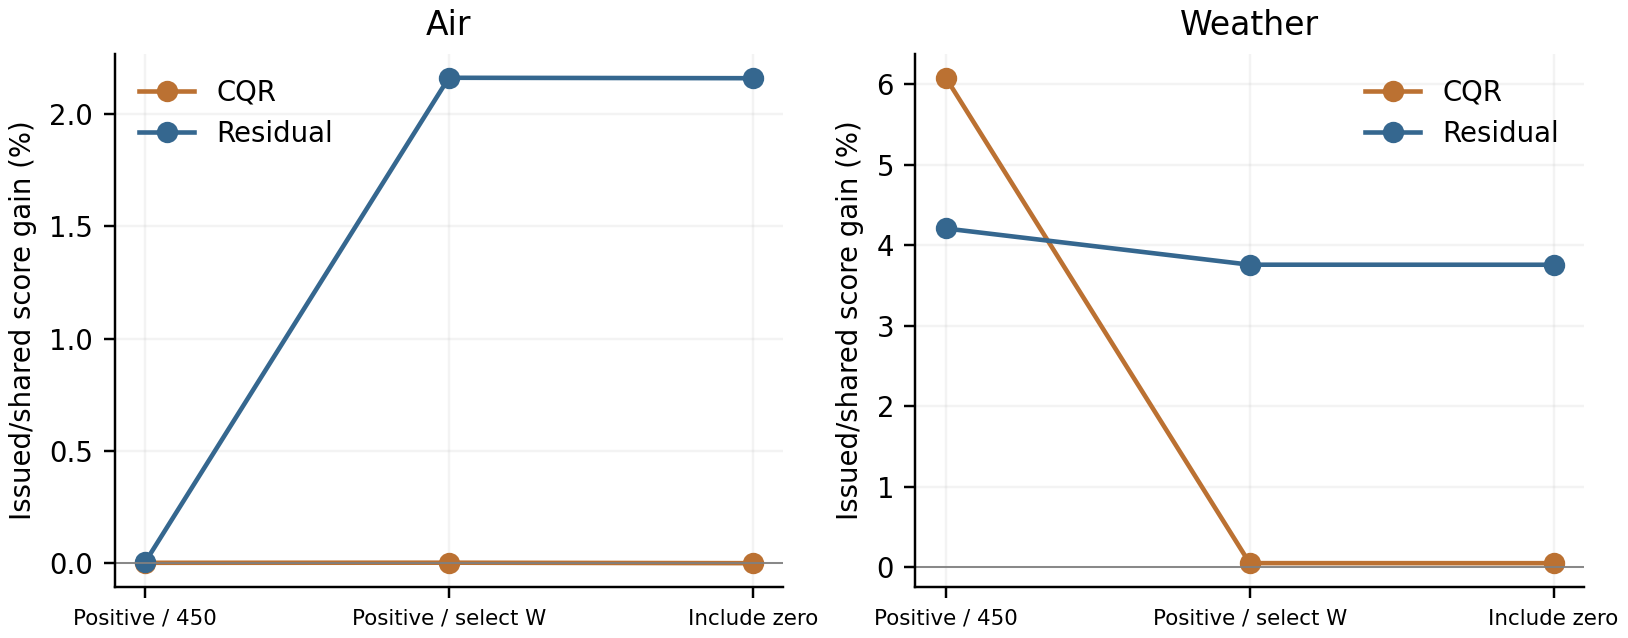
\includegraphics[width=\textwidth]{figures/positive_rates.png}
\caption{Post-review exploratory contrasts at $h=24$, four dependent pairs per
source. Positive rates include values as small as $10^{-6}$. Window selection uses
the fixed pre-test validation segment and the existing grid. The weather CQR gap
shrinks before zero is admitted; residual-score selection follows a different pattern.
These points compare selected configurations, not intrinsic state effects.}
\label{fig:core}\end{figure}

\section{Related work and comparison scope}
CQR uses predictive quantiles to define calibrated interval endpoints
\citep{romano2019cqr}; residual scaling supplies another established construction
\citep{lei2018distfree}. Online methods include ACI, adaptive aggregation, strongly
adaptive experts, PID, decaying-step optimization and optimistic updating
\citep{gibbs2021aci,zaffran2022acits,gibbs2024dtaci,bhatnagar2023saocp,
angelopoulos2023pid,angelopoulos2024decay,areces2025online,hu2026cop}.
Our primary contrasts hold the neural forecasts fixed while changing these components.
Declared implementation variants and their source checks are in \ref{app:rules}.

\citet{adler2025calibration}, published at ICLR 2026, examine native TSFM calibration,
prediction heads and rollout. Distribution-aware conformal prediction
\citep{schweizer2026dcp} already separates probabilistic predictors from scores.
We investigate a different comparison: whether changing the score changes the
apparent delayed-state benefit after rate and memory controls, and which native-band
benefits survive common support and asymmetric residual constructions. Foundation-model
conformal inference \citep{achour2025fm}, direct volatility modeling
\citep{cho2026volatility} and hidden-state-conditioned calibration
\citep{zhu2025afocp} provide related approaches; hidden representations are unavailable
in the forecast archives used here.

AcMCP models multi-step error autocorrelation and provides ACI/PID implementations
\citep{wang2026acmcp}. Its ACI uses a shared state. The delayed ACI analysis of
\citet{elhalabi2026delayed} establishes interleaving for issuing-state updates and
examines delay relative to residual memory, including rate dependence on residual
dynamics. Our window intervention changes the retained empirical score history on
the same forecast stream; it does not estimate that latent residual-memory scale.
Staggered integral control also treats delayed feedback \citep{cherenson2026staggered},
and O$^2$CP optimizes across horizons \citep{li2026o2cp}. We implement full configured
AcMCP-CSS on the complete weather subset and retain the wider PID comparison.

Three comparison types are kept distinct. Information contrasts hold the controller
fixed and change the score or interval construction. State contrasts at a fixed window
hold information and observation timing fixed, while allowing each state to select
its rate. Joint window selection compares deployable configurations; it does not
isolate state alone. AcMCP/PID versus native CQR is a complete-method comparison with
different information. These distinctions define the scope of the empirical contribution;
we do not infer new algorithmic validity guarantees from modified implementations.

\section{Causal calibration and explanatory accounting}
\subsection{Scores, observation timing and state}
At origin $t$, the frozen model emits a point forecast $m_t$ and ordered endpoints
$\ell_t,u_t$ for $y_t=Y_{t+h}$. At natural feedback lag $h$, calibration can use only
outcomes from origins $i\leq t-h$. The primary scores and inversions are
\begin{align}
s_t^{\rm R}&=|y_t-m_t|,& C_t^{\rm R}&=[m_t-q_t,m_t+q_t],\\
s_t^{\rm Q}&=\max(\ell_t-y_t,y_t-u_t),&
C_t^{\rm Q}&=[\ell_t-q_t,u_t+q_t].
\end{align}
CQR can have a negative threshold and shrink its native band. Reversed endpoints
are repaired to their midpoint and counted; coverage feedback uses the emitted
interval. Infinite scores remain infinite. The stored 0.1/0.9 band is a score input,
not an uncalibrated 90\% interval. No unrecorded tails are extrapolated. Additional
scale and midpoint controls are specified in \ref{app:details}.

Let $Q_p(\mathcal H_t)$ be the linearly interpolated empirical quantile of the last
$W$ observed, revealed scores. Rolling uses $q_t=Q_{1-\alpha}(\mathcal H_t)$, with
$\alpha=0.1$. ACI uses $q_t=Q_{1-a_t}(\mathcal H_t)$. For emitted-interval
miscoverage $e_i=\ind\{y_i\notin C_i\}$, the two established recursions are
\begin{align}
a_t^{\rm S}&=\clip_{[.001,.999]}\{a_{t-1}^{\rm S}+\gamma(\alpha-e_{t-h})\},\label{eq:shared}\\
a_t^{\rm I}&=\clip_{[.001,.999]}\{a_{t-h}^{\rm I}+\gamma(\alpha-e_{t-h})\}.\label{eq:issued}
\end{align}
They coincide at $h=1$. At larger $h$, issued updating has $h$ interleaved level
states; the common rolling history still couples their score information.
Both start at $a=\alpha$. At $\gamma=0$ they are the same Rolling method when
window and timing agree. Rolling continues to update its empirical distribution
even though it does not adjust the nominal level.

All trajectories exclude their first 600 forecast pairs from evaluation. Issuance
starts at $600+h-1$; validation uses $[600+h-1,1200-h+1)$ and testing starts at
1200, with state carried across the boundary. Thus every validation label is
available before test selection. Missing neural inputs are filled using past
observations only. Missing targets are excluded from score memory, error updates
and evaluation; issued phases continue without an increment. The full time-index
and missingness checks accompany the code.

\subsection{What the accounting explains}\label{sec:topology}
Clipping affects the usual telescoping coverage argument. For a revealed-error
update, write $r_k=a_{k+1}-a_k-\gamma(\alpha-e_k)$. Then
\begin{equation}\label{eq:identity}
\frac{1}{K}\sum_{k=1}^{K}e_k-\alpha
=\frac{a_1-a_{K+1}}{\gamma K}+\frac{\sum_{k=1}^{K}r_k}{\gamma K},\qquad\gamma>0.
\end{equation}
Bounded levels control the endpoint term but do not eliminate accumulated clipping.
For the delayed interpolation with raw update
$(1-\rho)a_{t-1}+\rho a_{t-h}+\gamma(\alpha-e_{t-h})$, define
$V_t=a_t+\rho\sum_{k=1}^{h-1}a_{t-k}$. Direct subtraction gives
\begin{equation}\label{eq:potential}
V_t-V_{t-1}=\gamma(\alpha-e_{t-h})+r_t.
\end{equation}
Shared and issued states correspond to $\rho=0,1$. The identity separates finite-time
endpoint and clipping contributions; unrevealed final outcomes are counted separately.
It is not a proof of conditional validity or a decomposition of all score differences.

Under a stationary differentiable miscoverage response with slope $g>0$, inactive
clipping and deterministic response feedback, linearized shared and issued errors
satisfy $x_t=x_{t-1}-\gamma g x_{t-h}$ and $x_t=(1-\gamma g)x_{t-h}$.
Their familiar stability ranges are
\begin{equation}\label{eq:stability}
0<\gamma g<2\sin\!\left(\frac{\pi}{4h-2}\right)\quad(\mathrm{shared}),
\qquad 0<\gamma g<2\quad(\mathrm{issued}).
\end{equation}
The first is the classical scalar delay-difference boundary
\citep{deger2017stability}; issued contraction per calendar step is
$|1-\gamma g|^{1/h}$. A wider stable gain range therefore need not mean faster
tracking. These approximations motivate rate controls. Empirical quantile jumps,
changing memory and clipping require the actual trajectory diagnostics in \ref{app:rates}.

\section{Experimental design}
\subsection{Evidence panels and analysis stages}
The original main panel has 31 series and four archived backbones (Chronos-2,
Chronos-Bolt, TimesFM and Moirai): 25 observed energy series, four constructed
series and two synthetic switches. Separate renewable and multi-horizon archives
provide supporting diagnostics. An original confirmation uses traffic and exchange
rates with two Chronos models, giving 16 pairs per horizon. These sources, time
units and archive limitations are specified in \ref{app:data}.

A further locally fixed protocol precedes numeric acquisition of two new sources:
Jena roof temperature and pressure in the first 3,600 hours of 2026, and PM2.5 at
two Beijing stations in the first 3,600 hours from 1 March 2013
\citep{jena2026weather,chen2017air}. The same two cached Chronos checkpoints generate
24 horizons at 2,976 consecutive origins, with context 512. Each test has 1,776
origins before excluding missing targets. Weather forecast targets are complete;
air-quality masks are retained. Four series and two models yield eight dependent
pairs, not eight independent replications.

Original and new-source confirmation choices were recorded before their respective
acquisitions. Later rate sensitivities, PV controls and the present positive-rate,
time-block and history analyses revisit inspected data and are exploratory.
Local timestamp/hash records are not external preregistration. Neither source novelty
within this calibration project nor recent observation dates establish exclusion
from neural pretraining. Detailed grids and chronology are in \ref{app:newprotocol}.

\subsection{Selection and comparisons}
The original matched ACI comparison selects each score's $(\gamma,W)$ from three
rates and $W\in\{200,450,900\}$. The new-source protocol nests the original three
rates, a wider grid with delay-scaled values, zero/small rates down to $10^{-6}$,
and finally window selection. Each state minimizes its own validation interval
score, with ties favoring smaller rate and then window. A separately selected
zero-rate Rolling control uses the same candidate windows. Test scores never
choose the search range. Positive-rate reanalysis uses only existing candidates,
holding $W$ fixed or selecting it before finally admitting zero.

Full AcMCP-CSS uses the pinned author's MA$(h-1)$ and cross-horizon regression,
all 24 horizons, history 600, and validation-selected learning rates. CSS is the
author's supported fitting option; its estimates need not equal default CSS-ML.
We add history 450 for a bounded sensitivity. Because the author's history parameter
also governs startup, this additional comparison uses a common post-startup
validation block $[900+h-1,1200-h+1)$, unchanged tests, and common histories
$\{450,600\}$ for CQR, Rolling and AcMCP/PID. Every evaluated scorecast is checked
finite. Fixed-600 and selected-history results answer complementary fairness
questions without presenting different fitting windows as equivalent algorithms.

On all 32 original PV pairs, the signed-error comparator uses
$[m_t+Q_{a_t/2}(Y-m),m_t+Q_{1-a_t/2}(Y-m)]$ with the same total-miscoverage state.
Each construction is tuned before and after common support projection
$[L,U]\mapsto[\max(0,L),\max(0,U)]$. Projection leaves each candidate's raw feedback
trajectory unchanged, isolating emitted-interval geometry. For a nonnegative target
it cannot increase interval score or lose a covered observation. In addition to
actual zero/positive groups, an issue-time grouping uses whether $m_t$ exceeds
the median of the first 600 forecasts. Its threshold never uses test outcomes.

\subsection{Metrics and temporal resolution}
For $[L,U]$, we use the proper interval score
\begin{equation}
\IS_\alpha=(U-L)+\frac{2}{\alpha}(L-y)_++\frac{2}{\alpha}(y-U)_+,
\end{equation}
alongside coverage and local absolute coverage error over 150-origin windows
\citep{winkler1972,gneiting2007proper}. Missing targets are excluded from each
window's denominator. Paired score gain is $100(1-\IS_A/\IS_B)$; ratios and gains
are calculated within each model--series pair before averaging, with equal source
weight for equal-sized confirmation panels. A positive local-error improvement
means the comparator's error minus the candidate's, in percentage points.

Three consecutive 592-origin test blocks reveal temporal heterogeneity without
reselecting models. Block-local windows stay within each block. The main-panel
bootstrap and dependence checks remain in the supplementary records; confirmation
pair counts and tiny score differences are descriptive, not independent-replication
confidence statements. We report score, overall coverage and local error together.

\section{Results}
\subsection{RQ1: What predictive-information benefits survive stronger controls?}
Across 124 main-panel pairs, default CQR--ACI improves score by 13.57\% relative
to default symmetric residual--ACI. Tuning both methods reduces the paired benefit
to 9.98\%. The latter is recomputed from every prediction archive and all nine
candidate settings for each score. Native-scale and midpoint controls, the full
original method table and family heterogeneity remain in \ref{app:details} and
\ref{app:earlierdiagnostics}; the default CQR benefit is 6.03\% after excluding PV.
On traffic/exchange rates, holding COP fixed gives native-score benefits of
12.27\%, 14.66\% and 22.16\% at $h=1,6,24$, respectively. Magnitudes depend on the
controller and panel; the comparisons do not pool scores in incompatible units.

The PV controls test two simpler explanations for the large original solar result:
symmetric intervals and extension into impossible negative outputs. Table~\ref{tab:pvcontrols}
shows that the positive-output benefit declines from 12.77\% to 11.57\% after
common projection, and to 9.56\% against projected signed residuals. Native information
therefore retains value after both controls. Successive percentages have different
denominators and selected settings, so their differences are not additive causal
contributions. The original zero/positive score decomposition and all width and
miss-penalty terms remain in \ref{app:solarparts} and \ref{app:details}.

\begin{table}[!htbp]\centering\scriptsize
\caption{PV construction controls, all 32 pairs, validation-tuned. Gains are mean
paired CQR improvements over the named baseline (\%); coverages are percent.
High forecast is an issue-time observable prefix-median split.}
\label{tab:pvcontrols}\begin{tabular}{lllrrr}
\toprule
Support & Baseline & Group & CQR gain & Cov. CQR & Cov. base \\
\midrule
Raw & Residual & all & 20.51 & 89.72 & 89.34 \\
Raw & Residual & positive & 12.77 & 86.32 & 80.17 \\
Raw & Residual & forecast high & 14.70 & 87.03 & 82.91 \\
Nonnegative & Residual & all & 15.61 & 91.56 & 90.55 \\
Nonnegative & Residual & positive & 11.57 & 86.45 & 80.50 \\
Nonnegative & Residual & forecast high & 12.41 & 87.07 & 83.04 \\
Nonnegative & Signed & all & 10.86 & 91.56 & 91.40 \\
Nonnegative & Signed & positive & 9.56 & 86.45 & 80.09 \\
Nonnegative & Signed & forecast high & 9.26 & 87.07 & 84.59 \\
\bottomrule
\end{tabular}
\end{table}

\subsection{RQ2: What does adaptation add after rate and memory selection?}\label{sec:rates}
The earlier traffic/exchange-rate sensitivity reduced the CQR issued/shared gain
at $h=24$ from 8.43\% to 0.99\% after widening the rate range. On the new-source
confirmation, small/zero rates remove the air-quality gap but leave 6.08\% on
weather at $W=450$. Adding window selection lowers that gap to about 0.05\%
(Table~\ref{tab:newconfirm}). This is why a rate-only explanation is incomplete.

\begin{table}[!htbp]\centering\small
\caption{Locked new-source confirmation at $h=24$. Mean paired issued/shared
score gain (\%), four pairs per source. Only the last column selects memory.}
\label{tab:newconfirm}\begin{tabular}{llrrrr}
\toprule
Source & Score & Original & Wide & Zero/small & Window \\
\midrule
Air quality & Residual & 15.04 & 3.08 & 0.00 & 2.16 \\
Air quality & CQR & 10.59 & 0.23 & 0.00 & 0.00 \\
Weather & Residual & 7.82 & 4.32 & 4.21 & 3.76 \\
Weather & CQR & 9.21 & 6.11 & 6.08 & 0.05 \\
\bottomrule
\end{tabular}
\end{table}

Does this attenuation merely select the identical zero-rate method? The post-review
positive-rate controls separate those possibilities (Table~\ref{tab:positive}).
Weather CQR has a 6.080\% gap with positive rates at $W=450$, 0.052\% when
positive-rate methods select their window, and 0.052\% after zero is admitted
at the displayed precision. The window-dependent attenuation therefore occurs
without exact zero. However, six of eight issued and seven of eight shared CQR
positive-rate selections use $10^{-6}$; positivity alone does not establish
substantial feedback. The result describes the tested search and its rolling limit.

\begin{table}[!htbp]\centering\small
\caption{Exploratory positive-rate decomposition, $h=24$, mean paired state gain
(\%). The first three columns exclude zero. ``Select $W$'' uses 200, 450 and 900;
``Add zero'' differs only by admitting zero. Tiny rates remain eligible.}
\label{tab:positive}\begin{tabular}{llrrrr}
\toprule
Source & Score & $W=450$ & $W=900$ & Select $W$ & Add zero \\
\midrule
Air & CQR & 0.002 & -0.003 & 0.002 & 0.000 \\
Air & Residual & 0.004 & 2.161 & 2.161 & 2.159 \\
Weather & CQR & 6.080 & 0.052 & 0.052 & 0.052 \\
Weather & Residual & 4.208 & 0.001 & 3.759 & 3.758 \\
\bottomrule
\end{tabular}
\end{table}

Residual scores show why selected configurations must also be inspected. On weather,
their state gap is essentially zero when both use $W=900$, yet is 3.759\% after
independent window selection. The shared residual method selects $W=450$ for both
pressure series while the issued method selects 900. The resulting test gap is
partly a difference in validation-selected memory, not a residual intrinsic state
effect. On air quality, allowing window selection also brings back a residual gap.
Larger validation searches need not improve every test result.

Table~\ref{tab:choices} exposes every final CQR choice. Six of eight pairs choose
the exact same zero-rate/window method. The two pressure pairs choose distinct
settings and retain small score differences. Seven of eight configurations in each
state select the largest allowed window; early and late validation select identical
settings for only three issued and four shared pairs. These boundary and stability
checks preclude interpreting the final mean as a precisely identified state effect.

\begin{table}[!htbp]\centering\scriptsize
\caption{Every final CQR pair at $h=24$, original full-validation selector. S/I
are shared/issued; C2 and Bolt are the two Chronos models. IS is in the respective
series' units. Same rolling means both rates are zero with the same window.
Air A/D denote Aotizhongxin/Dingling.}
\label{tab:choices}\begin{tabular}{lrrrrrrl}
\toprule
Pair & $\gamma_S$ & $W_S$ & IS$_S$ & $\gamma_I$ & $W_I$ & IS$_I$ & Selection \\
\midrule
Air A / C2 & 0 & 900 & 288.250 & 0 & 900 & 288.250 & Same rolling \\
Air A / Bolt & 0 & 450 & 319.915 & 0 & 450 & 319.915 & Same rolling \\
Air D / C2 & 0 & 900 & 238.382 & 0 & 900 & 238.382 & Same rolling \\
Air D / Bolt & 0 & 900 & 300.438 & 0 & 900 & 300.438 & Same rolling \\
Pressure / C2 & 0.0001 & 900 & 21.442 & 0.002 & 900 & 21.437 & Distinct \\
Pressure / Bolt & 0 & 900 & 20.385 & 0.00208 & 900 & 20.348 & Distinct \\
Temperature / C2 & 0 & 900 & 15.152 & 0 & 900 & 15.152 & Same rolling \\
Temperature / Bolt & 0 & 900 & 14.491 & 0 & 900 & 14.491 & Same rolling \\
\bottomrule
\end{tabular}
\end{table}

Against separately window-selected Rolling CQR, the final issued CQR mean score
gain is zero on air quality and 0.04\% on weather at $h=24$; weather coverage is
89.43\% versus 89.51\%. The earlier traffic/exchange-rate comparison likewise
gives only 0.17\% mean gain over Rolling. COP instead has a 2.90\% higher score
there but better overall and local coverage. The correct interpretation requires
the reliability comparisons in RQ3, rather than a score-only ranking.

\paragraph{A common-history AcMCP check.}
The original full AcMCP-CSS comparison used history 600 against CQR allowed to
select 200/450/900. At $h=24$ its mean paired score ratio to selected Rolling was
1.147, with 87.54\% coverage. The extra comparison in Table~\ref{tab:history}
restricts all methods to common history options and a common post-startup validation
segment. It includes every weather pair and the no-scorecast PID ablation.
With common history 600, AcMCP's score ratio is 1.172; selecting 450/600 gives
1.164, with 89.18\% coverage. Fixed 450 scores better on the test than the joint
selector, another reminder that validation search is not a test oracle. Issued
CQR remains close to Rolling, whereas shared CQR has a 1.039 score ratio under
the joint selector. Thus the nearly zero original state gap does not persist
under every history and validation choice.
The history check is a bounded complete-configuration sensitivity; native CQR and
signed-error methods still receive different predictive information. All horizons,
selected rates, success counts and source checks are retained in \ref{app:focused}.

\begin{table}[!htbp]\centering\small
\caption{Common-history weather comparison at $h=24$, four pairs. All rows use
the same post-startup validation block and unchanged test origins. Each IS ratio
uses its matched Rolling method within that history search; coverage is percent
and Local is percentage points.}
\label{tab:history}\begin{tabular}{llrrr}
\toprule
History & Method & IS ratio & Coverage & Local \\
\midrule
450 & Rolling-CQR & 1.000 & 89.32 & 6.33 \\
450 & CQR-shared & 1.136 & 83.22 & 8.96 \\
450 & CQR-issued & 1.000 & 89.27 & 6.34 \\
450 & AcMCP-CSS & 1.138 & 89.18 & 6.45 \\
450 & PID-no-scorecast & 1.061 & 88.20 & 6.49 \\
600 & Rolling-CQR & 1.000 & 89.44 & 6.75 \\
600 & CQR-shared & 1.039 & 87.43 & 7.42 \\
600 & CQR-issued & 1.000 & 89.43 & 6.74 \\
600 & AcMCP-CSS & 1.172 & 89.27 & 6.27 \\
600 & PID-no-scorecast & 1.067 & 88.37 & 6.43 \\
450/600 & Rolling-CQR & 1.000 & 89.44 & 6.75 \\
450/600 & CQR-shared & 1.039 & 87.43 & 7.42 \\
450/600 & CQR-issued & 1.000 & 89.43 & 6.74 \\
450/600 & AcMCP-CSS & 1.164 & 89.18 & 6.48 \\
450/600 & PID-no-scorecast & 1.065 & 88.60 & 6.24 \\
\bottomrule
\end{tabular}

\end{table}

\subsection{RQ3: Which reliability gains and deficits remain?}\label{sec:rolling}
Adaptive levels can supply local reliability even when average-score improvements
are small. On weather at $h=1$, adaptive CQR improves mean paired score by 0.36\%
while reducing average local coverage error from 3.15 to 1.43 percentage points.
Table~\ref{tab:localpairs} shows every pair and every test block. Both pressure
series and Chronos-2 temperature improve local error in all three blocks, despite
mixed signs for their score gains. Chronos-Bolt temperature selects the same
zero-rate rolling configuration and has identical results. This is neither a
universal benefit nor an effect of issued versus shared states, which coincide
at one step.

\begin{table}[!htbp]\centering\scriptsize
\caption{Weather $h=1$: adaptive CQR versus selected-window Rolling. Gain is
paired score improvement (\%). Whole-test local errors and their block improvements
are percentage points; positive block values favor ACI. All configurations are
selected before testing.}
\label{tab:localpairs}\begin{tabular}{lrrrrrr}
\toprule
Pair & Score gain & Local roll & Local ACI & Early & Middle & Late \\
\midrule
Pressure / C2 & +1.77 & 4.51 & 1.45 & +2.83 & +3.88 & +3.81 \\
Pressure / Bolt & +0.20 & 3.75 & 0.86 & +2.76 & +2.58 & +3.01 \\
Temperature / C2 & -0.54 & 2.14 & 1.19 & +1.08 & +1.05 & +1.15 \\
Temperature / Bolt & +0.00 & 2.21 & 2.21 & +0.00 & +0.00 & +0.00 \\
\bottomrule
\end{tabular}
\end{table}

The benefit varies with horizon and source (Table~\ref{tab:tradeoff}). The complete
block-by-pair display in \ref{app:focused} shows where favorable averages conceal
different time periods. These descriptive slices identify the empirical extent
of the benefit; they do not establish that a measured drift variable caused it.
The average interval score rewards width and miss distance, whereas local coverage
error penalizes persistent deviations from the target frequency. Improvements on
one metric therefore need not have the same size or sign on the other.

The same distinction is visible for another method. In the common-history
sensitivity at $h=1$ and history 600, AcMCP-CSS has a score ratio of 1.023 but
local error of 2.09 percentage points, compared with Rolling's 3.44. PID reaches
1.86 points. These use the same later validation block and fixed history, so
their local gains are not compared with a differently tuned Rolling denominator.
Local-reliability value is therefore not exclusive to native CQR, and a slightly
worse average score need not make a feedback configuration uniformly inferior.

\begin{table}[!htbp]\centering\scriptsize
\caption{Whole-test tradeoffs for the original new-source selector, four pairs
per source. ACI denotes issued CQR (identical to shared at $h=1$); gain is relative
to selected-window Rolling CQR. Coverage is percent and Local is percentage points.}
\label{tab:tradeoff}\begin{tabular}{lrrrrrr}
\toprule
Source & $h$ & Gain & Cov. roll & Cov. ACI & Local roll & Local ACI \\
\midrule
Air & 1 & -0.77 & 90.59 & 90.55 & 2.32 & 1.94 \\
Air & 6 & +0.00 & 89.65 & 89.65 & 4.85 & 4.85 \\
Air & 24 & +0.00 & 89.84 & 89.84 & 6.37 & 6.37 \\
Weather & 1 & +0.36 & 89.37 & 89.44 & 3.15 & 1.43 \\
Weather & 6 & -0.18 & 90.27 & 90.44 & 2.91 & 2.91 \\
Weather & 24 & +0.04 & 89.51 & 89.43 & 6.03 & 6.01 \\
\bottomrule
\end{tabular}
\end{table}

Exact clipping accounting explains one concrete coverage cost in the older
traffic/exchange-rate panel. Original-grid shared CQR has 2.150 percentage points
of revealed-test excess miscoverage: 2.117 from clipping and 0.033 from the endpoint
term. With scaled rates, clipping falls to 0.336 while the endpoint term rises to
0.681. Smaller rates suppress one cost while increasing a finite-time adaptation
term. The full identity and controlled stability/tracking simulations are in
\ref{app:rates}; this accounting does not assign every score change to instability.

PV exposes a different reliability deficit. Under the strongest construction
control in Table~\ref{tab:pvcontrols}, CQR covers 91.56\% overall but only 86.45\%
of positive targets. The issue-time high-forecast group has a 9.26\% score gain
against projected signed residuals, yet only 87.07\% coverage. Projection can
newly cover zero outputs when both raw endpoints were negative, improving overall
coverage without resolving positive-output reliability. Thus the retained native
information benefit and the retained operational gap are simultaneous findings.

\section{Discussion and limitations}
The evidence supports a sequence of evaluation decisions. Establish native-information
value under matched controllers and plausible interval geometry. Then compare
feedback updates with selected-window Rolling, separating a common-window state
contrast from a joint configuration-selection contrast. Finally inspect local and
observable-group reliability. This sequence distinguishes three outcomes observed
here: surviving native-band benefits, a window-sensitive state-score difference
that becomes practically small, and local benefits that average scores understate.

The zero-rate result has a precise interpretation. Six pairs select the same
method, so equality is mathematically expected; the empirical finding is that
validation chooses that method and it remains competitive on later observations.
The positive-only controls show that exact degeneracy is not the sole explanation
for the weather attenuation, but tiny selected rates and window boundaries remain
important. The residual fixed-window versus selected-window contrast further
shows how a favorable apparent state gap can arise from different memory choices.
These observations guide fair comparisons without providing a universal controller
selection rule.

Generality remains limited. Weather comes from one site and two variables; air
quality uses two correlated stations, with two models and relatively short tests.
The panels include dependent energy series and constructed switches. New-source
choices were locked locally, whereas the positive-only, block and extra history
analyses use inspected data. All selectors and negative results are retained, but
these sensitivities are not additional independent confirmations. Broader uninspected
deployments would be needed to validate a practical adaptation-selection rule.

Finite search boundaries also matter. Maximum-window selections are frequent, and
the extra AcMCP comparison covers histories 450/600 with CSS and a fixed integrator
configuration. It does not optimize every AcMCP setting or implement O$^2$CP.
Complete-method rankings cannot isolate controller quality. Original historical
checkpoint metadata remain incomplete; exact spot checks and paired forecasts
support the calibration comparison but do not prove training-data exclusion.
The new archives retain checkpoint hashes and generation details. The default
CPU artifact reruns calibration; optional R fitting and neural generation have
separate dependencies and declared scope.

Finally, overall or local frequency diagnostics do not establish conditional coverage,
and lower interval score does not by itself quantify operational savings. The latter
would require a decision policy and explicit shortfall costs. Our contribution is
the tested attribution and reliability evidence at the stated scales, with those
boundaries visible rather than absorbed into a single method ranking.

\section{Conclusion}
Native predictive information retains benefits after matched tuning, support and
asymmetric-residual controls. Delayed-state score advantages depend on rate and
memory selection; the weather gap shrinks under positive-rate window controls
before exact zero is admitted. Near-rolling long-horizon scores coexist with
one-step local-reliability benefits from adaptive levels, while PV subgroup
undercoverage persists. Reporting these distinctions changes how calibration
methods should be compared and how their deployment evidence should be interpreted.

\section*{Data and code availability}
Supplementary Software S1 (\texttt{Supplementary\_Software\_S1.zip}) contains
164 forecast archives, source/protocol hashes, CPU reproduction, reference results
and an explicit \texttt{ARTIFACT\_MAP.md}. The entry point recomputes the 124-pair
headline, rate/window searches, PV controls and the new focused analyses. Cached
AcMCP replay uses supplied R fits; separate commands refit the full author algorithm.
Earlier unrerun controllers remain identified historical inputs. A repository URL
will be added after author upload; the prepared archive is the reviewer-access package.

\section*{Funding}
This work is supported by the National Natural Science Foundation of China
(Grant No. 62372409).
\section*{Declaration of competing interest}
The authors declare no competing interests.
\section*{Declaration of generative AI and AI-assisted technologies}
OpenAI Codex assisted with literature retrieval, code auditing, experiment implementation,
analysis and manuscript preparation. The authors remain responsible for reviewing the
methods, results, citations and final text.

\clearpage
\appendix

\section{Dataset and archive details}\label{app:data}
UCI consumer indices are 5, 37, 70, 103, 136, 168, 201, 234, 267 and 300 in the public
LSTNet-format electricity matrix. Alabama plant indices are 3, 21, 39, 57, 75, 93, 111
and 130. Main observed traces use the initial 8,000 raw observations, except the two
minute-level ETT channels (12,000) and ERCOT channels (16,000). The ETT columns are
ETTh1/OT, ETTh2/OT, ETTm1/HUFL and ETTm2/OT.

The two cross-consumer splices concatenate 1,500-point segments starting at raw offset
1,000 from clients (10,40,70,100) and (25,90,140,210). Seasonal constructions use clients
20 and 80, concatenating 1,200-point windows starting at offsets 4392, 8784, 13128 and
17544. They deliberately omit the intervening chronology. Synthetic series have length
6,000, seeds 1 and 7, AR coefficient 0.7, a sinusoid of period 200 and four piecewise
mean/innovation-scale regimes $(0,1),(0,2.2),(5,0.8),(-3,1.6)$.

The multi-horizon panel uses electricity clients 20 and 80, solar plants 10 and 30,
ETTh1/OT, the first cross-consumer splice, seasonal client 20 and synthetic seed 1.
Origins stop 24 steps before the raw-series end for every horizon, ensuring the same
origins within that panel. Public data sources are the LSTNet data repository\footnote{\url{https://github.com/laiguokun/multivariate-time-series-data}},
ETDataset\footnote{\url{https://github.com/zhouhaoyi/ETDataset}}, ERCOT historical
load\footnote{\url{https://www.ercot.com/gridinfo/load/load_hist}} and GEFCom2014.


\clearpage
\section{Detailed delayed-feedback results}
\begin{table}[h!]\centering\small
\caption{Multi-horizon comparison. Gains use the residual--ACI score at the same horizon.
Local error is in percentage points. Tuning never uses test labels.}
\label{tab:horizon}\begin{tabular}{lrrr}
\toprule
Horizon / method & Gain (\%) & Cov. (\%) & Local (pp) \\
\midrule
1 / residual/aci & 0.00 & 89.99 & 1.77 \\
1 / native-scale/aci & 12.91 & 90.01 & 1.31 \\
1 / cqr/aci & 14.35 & 90.03 & 1.39 \\
1 / cqr/pi-log & 14.94 & 90.02 & 1.50 \\
1 / cqr/saocp & 12.48 & 90.69 & 2.10 \\
1 / cqr/faci & 15.42 & 89.61 & 1.68 \\
1 / cqr/aci/tuned & 14.87 & 90.09 & 1.97 \\
6 / residual/aci & 0.00 & 89.46 & 2.44 \\
6 / native-scale/aci & -11.77 & 89.64 & 1.96 \\
6 / cqr/aci & 13.89 & 89.54 & 2.06 \\
6 / cqr/pi-log & 16.21 & 90.00 & 2.53 \\
6 / cqr/saocp & 5.26 & 84.09 & 6.13 \\
6 / cqr/faci & 15.50 & 86.74 & 3.81 \\
6 / cqr/aci/tuned & 15.47 & 89.74 & 3.13 \\
24 / residual/aci & 0.00 & 87.10 & 4.90 \\
24 / native-scale/aci & -52.27 & 87.32 & 4.50 \\
24 / cqr/aci & 13.15 & 87.34 & 4.52 \\
24 / cqr/pi-log & 17.09 & 89.96 & 4.86 \\
24 / cqr/saocp & 6.56 & 79.98 & 10.16 \\
24 / cqr/faci & 15.57 & 82.72 & 7.94 \\
24 / cqr/aci/tuned & 11.62 & 88.09 & 5.46 \\
\bottomrule
\end{tabular}
\end{table}


\clearpage
\section{Per-series primary comparison}
\begin{table}[h!]\centering\small
\caption{Default CQR--ACI compared with default residual--ACI, averaged over four backbones.}
\begin{tabular}{lrr}
\toprule
Series & Gain (\%) & Coverage (\%) \\
\midrule
ETTh1\_OT & 3.12 & 89.98 \\
ETTh2\_OT & 8.27 & 89.99 \\
ETTm1\_HUFL & 8.74 & 89.99 \\
ETTm2\_OT & 3.70 & 89.97 \\
electricity\_c103 & 5.21 & 89.97 \\
electricity\_c136 & 4.87 & 89.99 \\
electricity\_c168 & 5.90 & 89.93 \\
electricity\_c201 & 5.33 & 89.96 \\
electricity\_c234 & 6.61 & 90.00 \\
electricity\_c267 & 4.74 & 90.01 \\
electricity\_c300 & 17.21 & 89.91 \\
electricity\_c37 & 8.05 & 89.97 \\
electricity\_c5 & 8.43 & 89.95 \\
electricity\_c70 & 5.72 & 89.89 \\
ercot\_COAST & 0.77 & 90.01 \\
ercot\_ERCOT & -1.53 & 90.00 \\
ercot\_NORTH & 1.86 & 89.97 \\
seasonal\_elec\_c20 & 6.25 & 90.09 \\
seasonal\_elec\_c80 & 10.90 & 90.00 \\
solar\_p111 & 34.92 & 89.90 \\
solar\_p130 & 34.37 & 89.92 \\
solar\_p21 & 36.12 & 89.97 \\
solar\_p3 & 35.42 & 89.97 \\
solar\_p39 & 35.01 & 90.07 \\
solar\_p57 & 35.63 & 89.94 \\
solar\_p75 & 36.33 & 89.98 \\
solar\_p93 & 34.21 & 89.97 \\
spliced\_electricity\_4seg & 11.36 & 90.10 \\
spliced\_electricity\_4seg\_b & 13.27 & 90.02 \\
synthetic\_T6000 & 0.31 & 89.99 \\
synthetic\_T6000\_s7 & -0.42 & 90.02 \\
\bottomrule
\end{tabular}
\end{table}


\clearpage
\section{Confirmation controller diagnostics}\label{app:confirmation}
\begin{table}[htbp]\centering\scriptsize
\caption{Confirmation contrasts at $h=24$. Each row contains four series and two models.
Gain and median are paired interval-score improvements (\%); A is the first method in
the comparison and B the second. Coverage is in percent, target 90\%. Correlated pairs
are retained without interpreting the win count as independent replications.}
\label{tab:confirmation}\begin{tabular}{llrrrrr}
\toprule
Comparison & Family & Gain & Median & Wins & Cov. A & Cov. B \\
\midrule
Native / residual, COP & FX & 11.10 & 2.73 & 7/8 & 89.76 & 89.72 \\
Native / residual, COP & Traffic & 33.22 & 31.79 & 8/8 & 90.45 & 91.40 \\
Native / residual, issued ACI & FX & 3.79 & 1.06 & 8/8 & 89.03 & 89.10 \\
Native / residual, issued ACI & Traffic & 13.20 & 11.92 & 8/8 & 89.83 & 90.20 \\
Issued / shared, CQR & FX & 8.62 & 5.01 & 8/8 & 89.03 & 86.12 \\
Issued / shared, CQR & Traffic & 8.24 & 7.98 & 8/8 & 89.83 & 89.63 \\
\bottomrule
\end{tabular}

\end{table}

\begin{table}[h!]\centering\scriptsize
\caption{Unified comparison on the revisited panel at $h=24$. IS ratio averages
per-pair interval scores divided by that pair's residual rolling-quantile score;
lower is better. Family coverage is percent (target 90\%). Local is the family-balanced
150-origin absolute coverage error in percentage points; Singleton is percent.
Original rows retain locked-grid results, wide ACI and multi-step PID are subsequent
sensitivities. PI-log and SF-OGD retain fixed defaults, not tuned optima.}
\begin{tabular}{llrrrrr}
\toprule
Score & Controller & IS ratio & FX cov. & Traffic cov. & Local & Singleton \\
\midrule
Residual & Rolling & 1.000 & 87.48 & 89.58 & 6.77 & 0.000 \\
Residual & Shared, original & 1.063 & 87.75 & 88.51 & 5.66 & 0.000 \\
Residual & Issued, original & 0.929 & 89.10 & 90.20 & 6.58 & 0.000 \\
Residual & Shared, wide & 1.066 & 87.57 & 88.07 & 6.14 & 0.000 \\
Residual & Issued, wide & 0.939 & 88.53 & 89.72 & 6.57 & 0.000 \\
Residual & PI-log & 2.341 & 89.92 & 90.03 & 6.36 & 2.873 \\
Residual & SF-OGD & 5.146 & 90.18 & 90.03 & 6.63 & 4.356 \\
Residual & COP & 1.177 & 89.72 & 91.40 & 6.39 & 0.249 \\
Residual & Grouped ACI & 0.984 & 86.76 & 89.23 & 5.74 & 0.000 \\
Residual & Fixed-scale OGD & 1.096 & 86.11 & 90.50 & 7.14 & 0.344 \\
Residual & Implicit-delay & 1.057 & 86.05 & 90.03 & 6.98 & 0.000 \\
CQR & Rolling & 0.852 & 87.78 & 89.41 & 6.37 & 0.038 \\
CQR & Shared, original & 0.937 & 86.12 & 89.63 & 5.79 & 0.167 \\
CQR & Issued, original & 0.853 & 89.03 & 89.83 & 6.12 & 0.025 \\
CQR & Shared, wide & 0.860 & 88.02 & 89.53 & 6.21 & 0.031 \\
CQR & Issued, wide & 0.851 & 88.14 & 89.88 & 6.22 & 0.044 \\
CQR & PI-log & 2.048 & 90.04 & 89.98 & 6.06 & 3.011 \\
CQR & SF-OGD & 4.528 & 90.17 & 90.09 & 6.47 & 4.377 \\
CQR & COP & 0.879 & 89.76 & 90.45 & 5.57 & 0.028 \\
CQR & Grouped ACI & 0.904 & 87.45 & 89.67 & 5.62 & 0.018 \\
CQR & Fixed-scale OGD & 0.884 & 88.25 & 90.92 & 6.13 & 0.126 \\
CQR & Implicit-delay & 0.884 & 88.33 & 90.92 & 6.07 & 0.069 \\
Signed error & Multi-step PI & 1.163 & 86.89 & 89.22 & 6.68 & 0.024 \\
Signed error & Multi-step PID & 1.176 & 86.85 & 89.21 & 6.92 & 0.065 \\
\bottomrule
\end{tabular}

\end{table}


\clearpage
\section{Algorithm and integrity checks}\label{app:integrity}
The primary evidence concerns the archived forecasts, not a reranking of freshly
downloaded checkpoints. Offline spot checks reproduce the point and five quantile outputs
exactly at 21 selected origins per model across three main-panel series, for 84 checked
model--origin cases. For the two Chronos models, matching the original default batch
grouping of 256 contexts resolves differences observed with a seven-context batch.
TimesFM's checked outputs match the local 2.0 checkpoint through its Hugging Face adapter;
Moirai matches after its original quantile-rearrangement step. Current checkpoint hashes
and environment versions are recorded. These checks support archive provenance but
do not constitute a rerun of every forecast, and original checkpoint commits were not
stored with every archive. Possible pretraining exposure to
public benchmark data also precludes an assertion that all test series were unseen during
pretraining.


The executable checks test future-target perturbations at lags 1, 6 and 24, identical
evaluation masks, unit rescaling, exact stored-level selection, empirical quantile
agreement, interval-score arithmetic, finite behavior under zero-width forecasts and
the reference SAOCP expert recursion. Data validation independently reconstructs target
values from local raw-series loaders. Cache records include archive, protocol and code
hashes; aggregations reject stale code/protocol outputs.

Source implementations and licenses are retained for SAOCP/FACI and PID. The SAOCP
numerical check covers its nonnegative-score expert recursion, without validating a
theorem for signed or delayed extensions. \ref{app:rules} specifies controller
conventions; the artifact retains complete grids, failures and tail misses. Recorded
runtimes include possible compilation overhead and do not measure neural inference speed.

Additional checks cover clipping identities, COP source-recursion equivalence,
target/issue-time conversion, grouped feedback assignment and implicit proximal
optimality against an independent optimizer and subgradient conditions. Protocols
and exploratory amendments remain separately identifiable.

The asymmetric multi-step PID comparison matches the unmodified author implementation
over 24 horizons and four configured scorecasters, including future-target perturbations.
Check records and tolerances accompany the artifact. The later full AcMCP-CSS
weather comparison has 96 complete-trajectory checks and 60 independent scorecast refits.


\section{Matched implicit-update ablation}\label{app:implicit}
The implicit ablation exactly solves the proximal objective already considered by
\citet{hu2026cop}. With $p=1-\alpha$, pinball loss $\ell_p(u)=u(p-\ind\{u<0\})$,
and a fixed prefix-scaled step $\eta=\gamma(\max_{i<600}s_i-\min_{i<600}s_i)$
(range floored at $10^{-12}$), it uses
\begin{equation}\label{eq:prox}
 b_t=b_{t-1}+\eta(e_{t-h}-\alpha),\qquad
 q_t=\arg\min_q\left\{\frac{(q-b_t)^2}{2}
       +h\eta\,\widehat{\mathbb E}_t[\ell_p(S-q)]\right\}.
\end{equation}
The same 300-score convention supplies the empirical distribution. The matched OGD
ablation sets $q_t=b_t$. Both select from $\{0.005,0.02,0.05,0.1\}$ and these values
divided by $h$. The point of this control is to distinguish an implicit correction's
incremental value from the fixed scale and learning rate. The development screen also
retains half-step and explicit corrections; it did not validate a new algorithm.

The delay-scaled implicit correction in Equation~\eqref{eq:prox} has a plausible
stationary rationale. If the true and proxy CDFs have local densities $g>0$ and
$\widehat g\geq0$, its deterministic linearized delayed gain is
$c=\eta g/(1+h\eta\widehat g)$. With a correct slope it is below $1/h$ and hence
inside the classical shared-state stability boundary in Equation~\eqref{eq:stability}.
For fixed slopes, however, this is simply a smaller effective gain. It predicts no
automatic advantage over suitably tuned basic gradient updating, and the argument
does not cover changing empirical distributions or atoms.

The development screen evaluates 3,200 configuration instances, retaining every
setting. At $h=24$, implicit-delay CQR improves interval score by 2.54\% over issued
ACI and 2.08\% over delay-tuned COP, but only 0.23\% over matched fixed-scale OGD.
It fails the locally recorded continuation criterion of at least 3\% against both
strong baselines, even before further validation. On the subsequent confirmation
panel, its matched-OGD gain is $-0.08\%$: $-0.30\%$ for exchange rates and $0.14\%$
for traffic, with seven of 16 positive differences. We therefore retain this result
as a negative ablation, not a new main method. A more sophisticated update formula
is insufficient evidence of additional predictive information or better adaptation.



\section{Rate, delay and clipping diagnostics}\label{app:rates}
Figure~\ref{fig:ratesurface} uses the common ten-rate subset of the wide grid to
display the rate--delay sensitivity. It shows every listed rate's test behavior,
not a test-based selector. The original selected shared-state CQR score at each
horizon is a common per-pair denominator for both structures. The additional
delay-scaled rates also participate in selection and remain in the full result files.

\begin{figure}[htbp]\centering
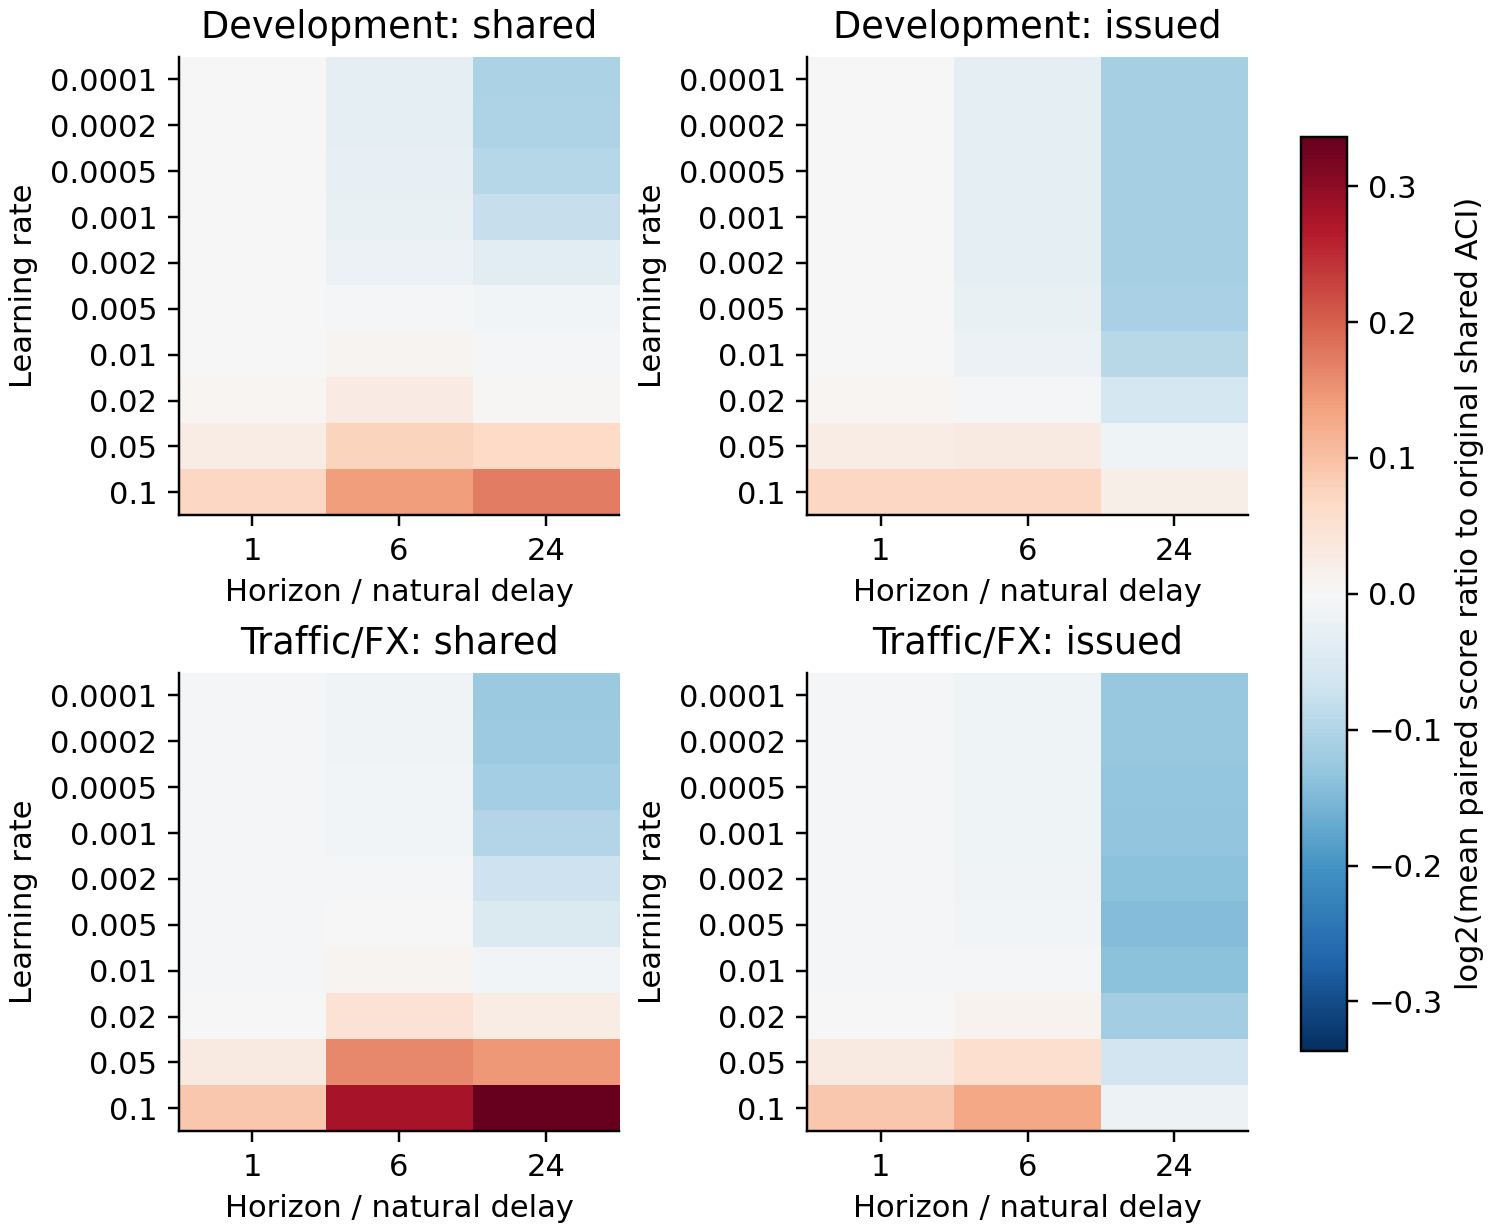
\includegraphics[width=\textwidth]{figures/rate_delay_surface.png}
\caption{CQR rate--delay surfaces. Color is the base-two logarithm of the mean
paired interval-score ratio to original-grid shared CQR; zero means equal score.
Positive values are worse. Development and revisited panels have 16 pairs each.
Validation selects configurations; the plotted test surface is descriptive.}
\label{fig:ratesurface}\end{figure}

\begin{table}[htbp]\centering\scriptsize
\caption{Exact revealed-test miscoverage decomposition, CQR, $h=24$, in percentage
points. Clip plus Endpoint equals Excess up to rounding. Each interval was issued
in the test segment and revealed by the last archive origin. The last 24 issued
test intervals are pending; their separately recorded contribution bounds the
difference from full issued-test coverage by $24/N_{\rm test}$.}
\begin{tabular}{lllrrr}
\toprule
Panel & Grid & State & Clip & Endpoint & Excess \\
\midrule
Development & original & shared & 1.801 & 0.004 & 1.804 \\
Development & original & issued & 0.023 & 0.393 & 0.415 \\
Development & scaled & shared & 0.043 & 0.398 & 0.441 \\
Development & scaled & issued & 0.023 & 0.611 & 0.633 \\
Development & wide & shared & 0.043 & 0.487 & 0.530 \\
Development & wide & issued & 0.023 & 0.642 & 0.664 \\
Traffic/FX & original & shared & 2.117 & 0.033 & 2.150 \\
Traffic/FX & original & issued & 0.135 & 0.461 & 0.596 \\
Traffic/FX & scaled & shared & 0.336 & 0.681 & 1.017 \\
Traffic/FX & scaled & issued & 0.135 & 0.863 & 0.998 \\
Traffic/FX & wide & shared & 0.336 & 0.909 & 1.245 \\
Traffic/FX & wide & issued & 0.182 & 0.834 & 1.016 \\
\bottomrule
\end{tabular}

\end{table}

For the controlled simulations, the response is prescribed as
$M_t(a)=\clip\{0.1+g(a-a_t^*),0,1\}$, with $g\in\{1,4\}$ and $h\in\{1,6,24\}$.
Runs contain 12,000 steps. Stationary runs use effective gains at 0.5 and 1.2 times
the shared linear boundary. Tracking runs use $a_t^*=0.1,0.2,0.06$ in three
4,000-step segments and the original three rates plus their delay-scaled versions.
Deterministic response feedback and Bernoulli feedback are kept distinct, with
20 fixed seeds for the latter, yielding 1,764 controller runs. In the deterministic
$h=24,g=4,\gamma=0.005$ tracking example, mean absolute state error over the first
500 steps after both changes is 0.0198 for shared and 0.0978 for issued updating.
This is a specified-response illustration, not a forecast score or a causal diagnosis
of all empirical losses.

\begin{figure}[htbp]\centering
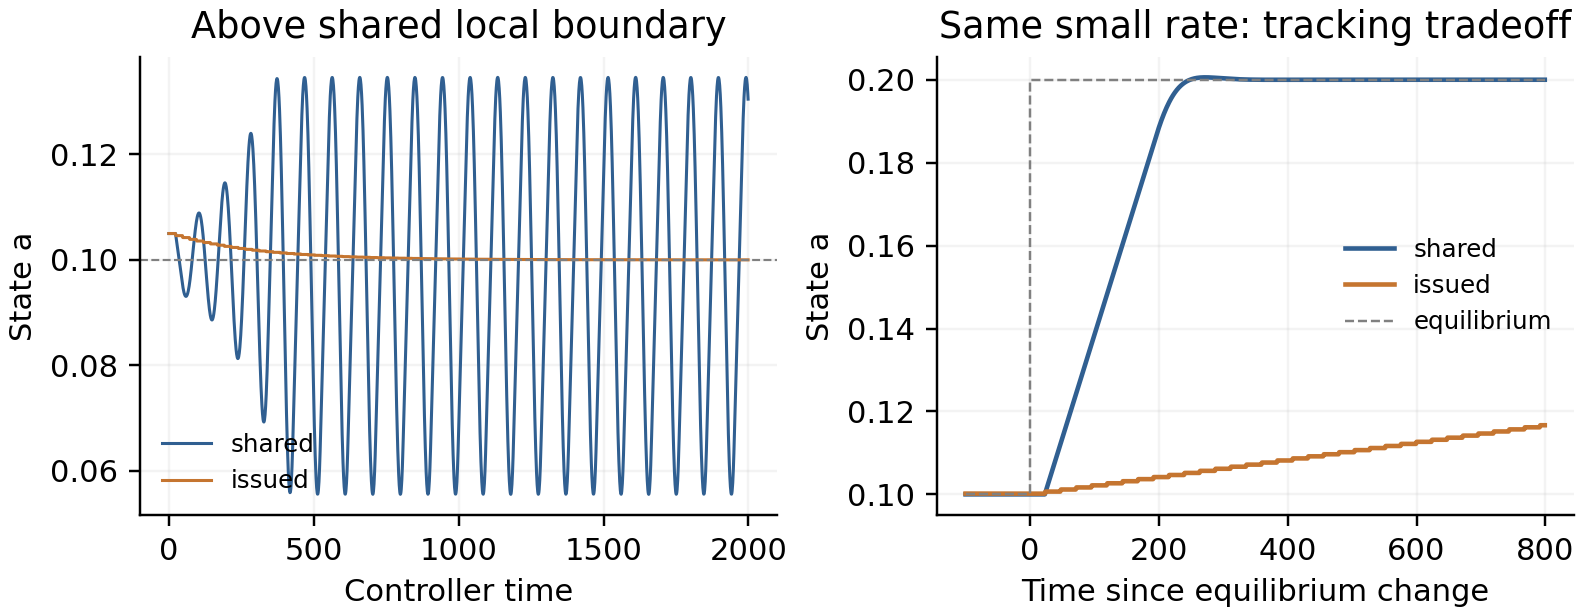
\includegraphics[width=\textwidth]{figures/controlled_dynamics.png}
\caption{Deterministic response illustrations at $h=24,g=4$. Left: effective gain
1.2 times the shared local boundary. Right: $\gamma=0.005$, below the boundary for
both states, following an equilibrium change. State clipping and response saturation
are explicit; the trajectories illustrate stability and tracking, not coverage guarantees.}
\label{fig:dynamics}\end{figure}


\section{Photovoltaic score components}\label{app:solarparts}
\begin{table}[htbp]\centering\small
\caption{One-step PV interval-score components, averaged over the original 32 pairs.
IS equals Width plus Lower plus Upper, where the last two are the $2/\alpha$-weighted
miss-distance penalties. These means use the shared PV data units; the headline
relative gains are instead calculated per pair before averaging. All outcome-defined
groups are evaluation-only.}
\begin{tabular}{lllrrrr}
\toprule
Settings & Score & Group & IS & Width & Lower & Upper \\
\midrule
default & cqr & all & 2.629 & 1.766 & 0.555 & 0.308 \\
default & cqr & positive & 5.978 & 3.831 & 1.386 & 0.761 \\
default & cqr & zero & 0.498 & 0.454 & 0.025 & 0.020 \\
default & residual & all & 4.046 & 2.284 & 1.218 & 0.544 \\
default & residual & positive & 7.607 & 3.086 & 3.126 & 1.395 \\
default & residual & zero & 1.781 & 1.773 & 0.006 & 0.002 \\
tuned & cqr & all & 2.575 & 1.816 & 0.476 & 0.282 \\
tuned & cqr & positive & 5.888 & 4.017 & 1.183 & 0.688 \\
tuned & cqr & zero & 0.467 & 0.417 & 0.027 & 0.023 \\
tuned & residual & all & 3.240 & 1.987 & 0.820 & 0.432 \\
tuned & residual & positive & 6.775 & 3.626 & 2.066 & 1.082 \\
tuned & residual & zero & 0.991 & 0.945 & 0.027 & 0.019 \\
\bottomrule
\end{tabular}

\end{table}
Each pair's all-observation score and coverage is reconstructed by weighting its
zero- and positive-output components by their own sample fractions. This check is
performed before any averaging across plants and models. There are no negative
targets in this evaluated PV panel. The original default and validation-tuned
overall scores are reproduced from the archived predictions before decomposition.


\section{Additional sensitivities}\label{app:sensitivity}
\subsection{Scale mismatch can amplify interval widths}
Normalization is helpful when the predicted scale tracks error size. It can also amplify
historical mistakes. For positive scales, a native-normalized residual interval has width
\begin{equation}\label{eq:ratio}
 2\tilde b_t\,Q_{1-a_t}\!\left(\{|y_i-m_i|/\tilde b_i:i\in\mathcal H_t\}\right).
\end{equation}
If more than the upper-tail fraction of the calibration history has error magnitude $c$
and scale $\varepsilon$, its empirical threshold can approach $c/\varepsilon$. A later
scale $B$ then produces width $2Bc/\varepsilon$. A relative floor keeps the expression
finite, but does not eliminate a large historical-to-current scale ratio. Additive CQR
does not have this particular multiplicative amplification mechanism, although it can
still perform poorly when the base endpoints or update rule are unsuitable.

This argument does not establish that every normalization loss is caused by exact zero
bands. Both scale transitions and very small but nonzero widths matter. We therefore
retain all failures, record floor activation and score extremes, and avoid a test-dependent
score cap. Nor does the argument establish that a proposed regularizer must improve
prediction: the validation and test experiments must decide that question.

\subsection{Normalization failures and unsuccessful selection}
At $h=24$, native-scale ACI has a mean gain of $-52.27\%$, despite a 12.91\% gain on
the same panel at $h=1$. Large losses occur on the Chronos-Bolt solar series and on
constructed scale switches, as well as smaller losses elsewhere. For example, its
interval-score increase on Chronos-Bolt/solar-p10 is 286.35\% relative to residual--ACI.
These cases are consistent with historical-to-current scale mismatch in
Equation~\eqref{eq:ratio}; exact zero bands are not required. The artifacts include
width-floor activation rates and normalized-score extremes for every trace.

Regularized normalized CQR does not reliably fix the problem. Across all three horizons,
its mean gains range from $-12.50\%$ at $\lambda=0$ to $-9.65\%$ at $\lambda=1$ for the
reported endpoint choices, compared with 13.80\% for additive CQR--ACI. The validation
selector increases the main-panel gain from 13.57\% to 13.72\%, but its multi-horizon
mean is 13.36\%, below fixed CQR--ACI. We retain this failed hypothesis instead of
expanding the selector grid on the test results. Prefix-based selection remains causal,
but a causal procedure need not transfer well across later regimes.

\subsection{Nominal levels, rearrangement and native-output provenance}
The primary CQR--ACI benefit persists at 80\% and 95\% calibrated targets
(Table~\ref{tab:sensitivity}). Omitting quantile rearrangement changes the primary mean
gain from 13.57\% to 13.56\%. The main conclusion is therefore not driven by sorting,
although sorting matters more for some individual normalized-score configurations.

\begin{table}[htbp]\centering\small
\caption{CQR--ACI sensitivity, using default residual--ACI at the same nominal level as
the denominator. Dense archives are a repeated-output sensitivity, not new independent data.}
\label{tab:sensitivity}\begin{tabular}{lrrr}
\toprule
Panel / miscoverage & Pairs & Gain (\%) & Cov. (\%) \\
\midrule
main-a0.2 & 124 & 9.85 & 80.01 \\
main-a0.1 & 124 & 13.57 & 89.98 \\
main-a0.05 & 124 & 14.00 & 94.90 \\
dense-a0.1 & 93 & 13.80 & 89.98 \\
gefcom-a0.1 & 39 & 19.63 & 89.99 \\
\bottomrule
\end{tabular}
\end{table}

The genuine stored 0.1--0.9 native bands achieve average main-panel coverage of 81.89\%
(Chronos-2), 87.04\% (Chronos-Bolt), 81.96\% (Moirai) and 77.57\% (TimesFM), against
their 80\% nominal mass. These values include both overcoverage and undercoverage.
They cannot substantiate a claim that all models' native 90\% intervals under-cover.

The dense archive requires additional care. TimesFM still stores only the five original
levels, so it supplies no genuine 0.05--0.95 comparison. Chronos-Bolt's stored 0.05 and
0.95 outputs equal its 0.1 and 0.9 outputs on approximately 99.86\% of rows after
rearrangement; requesting more levels did not create independent tail information.
Chronos-2's stored 0.05--0.95 band attains 91.69\% coverage at a nominal 90\%.
We therefore do not use the dense files to claim exact full-distribution CRPS or a
universal native 90\% calibration result.

\setlength{\bibsep}{4pt}


\section{Controller implementation details}\label{app:rules}
\subsection{One-step and delayed rule variants}
We compare seven rules using the same score streams and observation schedule.
\begin{enumerate}
\item \emph{Split}: a fixed empirical $(1-\alpha)$ quantile of the initial 600 scores.
\item \emph{Rolling}: an empirical $(1-\alpha)$ quantile of the latest $W=450$ revealed scores.
\item \emph{Clipped ACI}: replace $\alpha$ in the rolling quantile by $a_t$, updated as
\begin{equation}\label{eq:aciappendix}
 a_t=\clip_{[0.001,0.999]}\{a_{t-1}+\gamma(\alpha-e_{t-d})\},\qquad \gamma=0.02,
\end{equation}
where $e_i=\ind\{y_i\notin C_i\}$ and the update is applied only after an issued interval's
outcome becomes available. The equation suppresses idle steps before that event.
\item \emph{SF-OGD adaptation}: with $M=\max_{i<600}|s_i|$, update the threshold by
$q\leftarrow q-Mg/\sqrt{\sum g^2}$, where $g=\alpha-e$. We initialize at the prefix
quantile and allow signed thresholds. This coverage-gradient implementation is described
explicitly rather than claimed identical to every tie/projection convention in the
published wrapper \citep{bhatnagar2023saocp}.
\item \emph{PI-log adaptation}: a proportional threshold update and logarithmic tangent
integrator inspired by \citet{angelopoulos2023pid}. With $k$ revealed post-initialization
errors and $E_k=\sum_{j=1}^k(e_j-\alpha)$,
\begin{equation}\label{eq:pi}
 z_k=z_{k-1}+\gamma M(e_k-\alpha),\qquad
 q_k=z_k+M\tan\!\left(E_k\frac{\log(k+2)}{k+1}\right).
\end{equation}
The tangent saturates to signed infinity outside $(-\pi/2,\pi/2)$. The initial $z$ is the
prefix quantile. We use a fixed prefix scale, omit scorecasting and retain our causal
delay convention; this is not full reference PID.
\item \emph{SAOCP adaptation}: the strongly adaptive coin-betting expert update from
the author implementation \citep{bhatnagar2023saocp}, with default lifetime multiplier 8
and prefix scale $\sqrt{3}M$. The accelerated residual-score implementation agrees
numerically with an independent driver of the original expert class. For signed CQR we
remove its nonnegative projection; with delayed feedback, experts process scores in
reveal order. These are declared extensions, without transferring the original theorem
to the modified setting.
\item \emph{FACI-R}: the author's FACI aggregation update with eight learning rates
$0.001\,2^j$, $j=0,\ldots,7$, fixed-share mixing and a rolling 450-score empirical survival
function. Unlike a full-history wrapper, this variant deliberately shares the rolling
history design. Its weighted level is inverted using the empirical inverted-CDF quantile.
\end{enumerate}
The first five rules use linear empirical quantile interpolation where applicable.
Consequently, ``split'' denotes the fixed-threshold comparator here; we do not assert
the exact finite-sample rank correction or exchangeability guarantee of textbook split
conformal prediction for these dependent streams.

For ACI, we separately select $(\gamma,W)$ from
$\{0.005,0.02,0.05\}\times\{200,450,900\}$ using only the validation prefix.
The score selector retains the declared default rule settings. We report fixed defaults
and tuned controls separately, rather than describing one untuned baseline as optimal.


\subsection{Optimistic and groupwise controls}
The exact COP reference recursion is checked numerically against the author's
implementation. Our delayed adaptation is distinct: at issue $t$, with $j=t-h$,
it uses the preceding 300 revealed scores, excluding $s_j$, to form the empirical
CDF $\widehat F_t$ and step scale $R_t=\max s-\min s$. After feedback starts, it updates
\begin{equation}\label{eq:cop}
 b_t=b_{t-1}+\eta_t(e_j-\alpha),\qquad
 q_t=b_t-\tfrac12\eta_t\{\widehat F_t(b_t)-(1-\alpha)\},\quad \eta_t=\ell R_t.
\end{equation}
It starts from the 0.9 quantile of the 600-score prefix; before the first issued
interval's feedback arrives, the threshold stays at that initial value.
Validation selects $\ell$ from $\{0.05,0.1,0.5,1\}$ and those values divided by $h$.
The divided-rate extension was added after inspecting the development panel and is
explicitly exploratory there. It was fixed before the confirmation evaluation.
Singleton repairs use actual emitted-interval feedback; the original COP guarantees
are not asserted for this delayed, repaired adaptation.

Grouped ACI is an established groupwise-calibration control \citep{vovk2005algorithmic}.
The grouping feature is native band width, with a threshold fixed at its median in
the first 600 forecasts; ties enter the low-width group. The development factorial
separates score memory, feedback state, both, or neither. Group memory retains 450
scores per group and falls back to global history with fewer than 20 observations.
Each revealed error updates the state assigned at its issue time. Confirmation uses
the version with both memory and state separated, with the same ACI rate grid.

The matched implicit-update control and its negative result are specified in
\ref{app:implicit}.


\subsection{Configured multi-step PID}
We also compare the asymmetric multi-step PID implementation supplied with AcMCP
\citep{wang2026acmcp,angelopoulos2023pid}. Its two tails target $\alpha/2$, retain the
author's zero internal initialization and warmup recursion, and use error-range-scaled
steps and the unbounded tangent integral correction. We set rolling history to 600,
$C_{\rm sat}=0.5$, and initialize $K_I$ to the maximum absolute error revealed in the
first 600 target-clock rows across horizons 1--24, rather than using the whole trace.
Validation selects the rate from $\{0.005,0.01,0.05,0.1\}$ and those rates divided by
$h$, jointly with no scorecaster, a rolling mean, the author's documented naive
scorecaster, or a declared least-squares AR(1). The latter clips the fitted coefficient
to $[-0.995,0.995]$, recalculates the intercept from sample means, and iterates $h$ steps.
It is a configured scorecaster, not the author's default or an AcMCP substitute.

An accelerated implementation reproduces the unmodified author recursion on one
1,000-origin electricity archive for all 24 horizons and four scorecasters, and passes
future-target perturbation checks. The benchmark evaluates all 32 development/revisited
pairs and all three horizons, totaling 2,560 configurations. Crossed endpoints are
collapsed to their midpoint for evaluation, while the internal tail-score feedback is
preserved for source fidelity. Infinite or invalid intervals receive infinite score
rather than being omitted. A separately selected no-scorecaster control is retained.



\section{Earlier family, rule and delay diagnostics}\label{app:earlierdiagnostics}
\subsection{One-step rule diagnostics}
Across the seven default rules, adding native information generally improves efficiency,
but the effects are not orders of magnitude apart (Figure~\ref{fig:rules}). FACI-R with
residuals already gains 8.57\% and has lower coverage, while residual SAOCP overcovers
on average. CQR--PI-log, CQR--SF-OGD and CQR--ACI have similar average interval scores
but different local errors. SF-OGD has the smallest mean local error among these three
one-step CQR variants. A universal assertion that the score renders the rule irrelevant
is therefore unsupported even before adding delayed feedback.

\begin{figure}[htbp]\centering
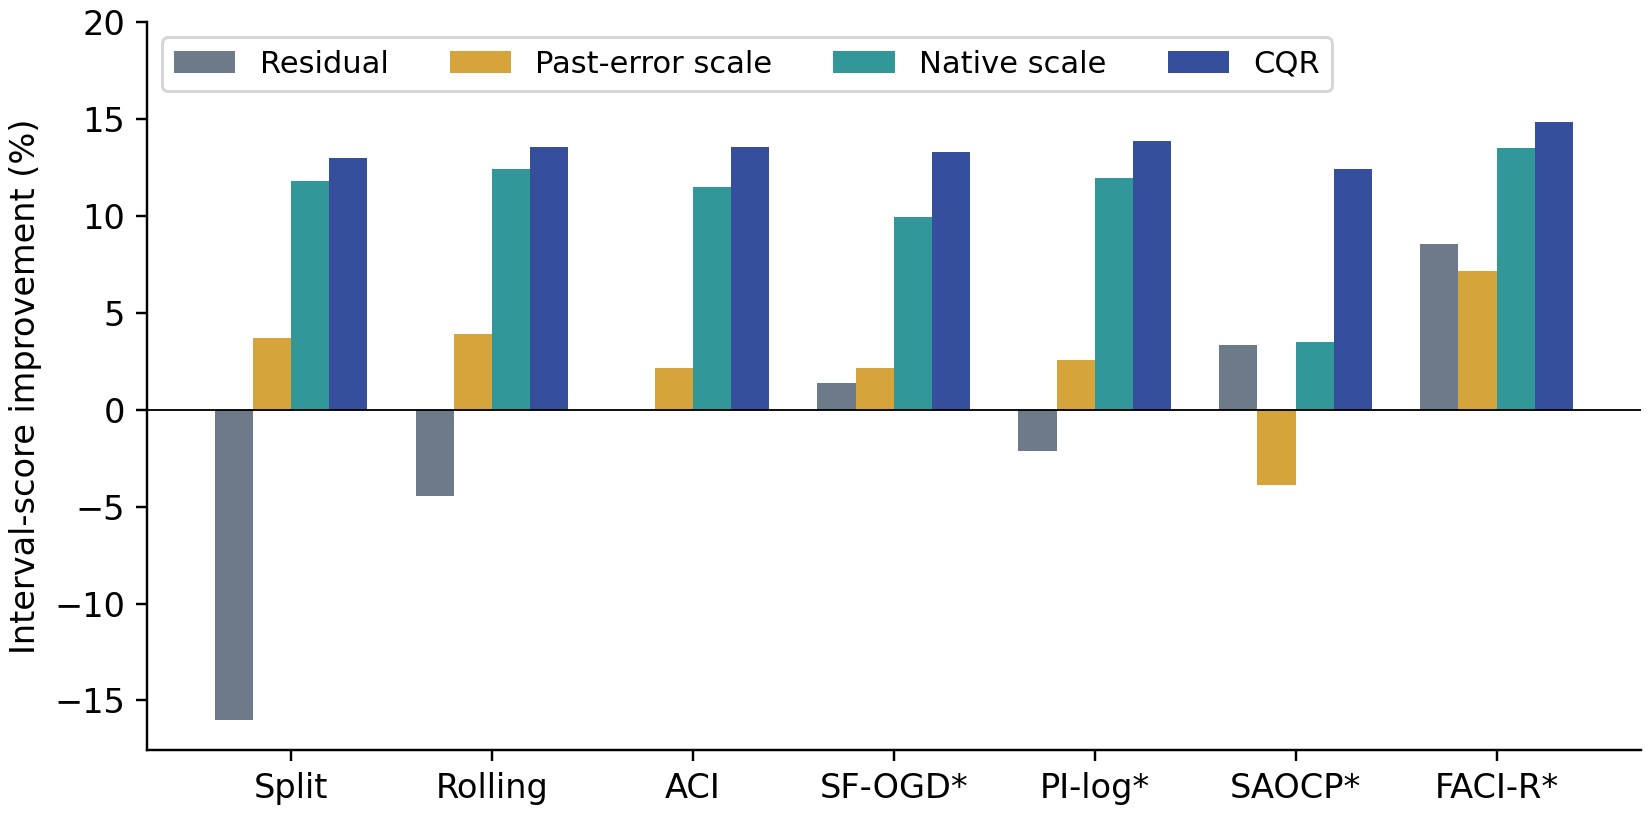
\includegraphics[width=\textwidth]{figures/score_rule.png}
\caption{Score--rule comparison on fixed one-step forecasts. Every gain uses the same
default residual--ACI denominator. Asterisks indicate the explicit adaptations described
in \ref{app:rules}; these labels do not claim equivalence to full original forecasting pipelines.}
\label{fig:rules}\end{figure}

\subsection{Benefits vary by family and persist on separate renewable series}
The mean CQR--ACI gain is 35.25\% on Alabama PV, 7.21\% on UCI loads, 5.96\% on ETT
and only 0.37\% on the three ERCOT loads (Table~\ref{tab:family}). The synthetic mean
is slightly negative. This heterogeneity is more informative than a pooled correlation
between a post-hoc volatility index and gains. Removing all eight PV series leaves
a 6.03\% gain, with descriptive interval $[4.25,7.88]\%$. Restricting to the 25 observed
series yields 15.16\%; that subset gives PV a larger relative weight. Leave-one-family-out
means remain positive, ranging from 6.03\% to 16.60\%.

\begin{table}[htbp]\centering\small
\caption{CQR--ACI gains by main-panel family. Intervals resample series within the listed
family and are descriptive; narrow intervals for correlated PV plants do not imply broad
geographic certainty. Small two- or three-series groups have especially limited precision.}
\label{tab:family}\begin{tabular}{lrrr}
\toprule
Family & Series & Gain (\%) & Descriptive 95\% CI \\
\midrule
Alabama PV & 8 & 35.25 & [34.75, 35.74] \\
Constructed seasons & 2 & 8.58 & [6.25, 10.90] \\
Constructed switches & 2 & 12.31 & [11.36, 13.27] \\
ERCOT & 3 & 0.37 & [-1.53, 1.86] \\
ETT & 4 & 5.96 & [3.41, 8.51] \\
Synthetic & 2 & -0.05 & [-0.42, 0.31] \\
UCI load & 10 & 7.21 & [5.53, 9.70] \\
\bottomrule
\end{tabular}
\end{table}
\begin{figure}[htbp]\centering
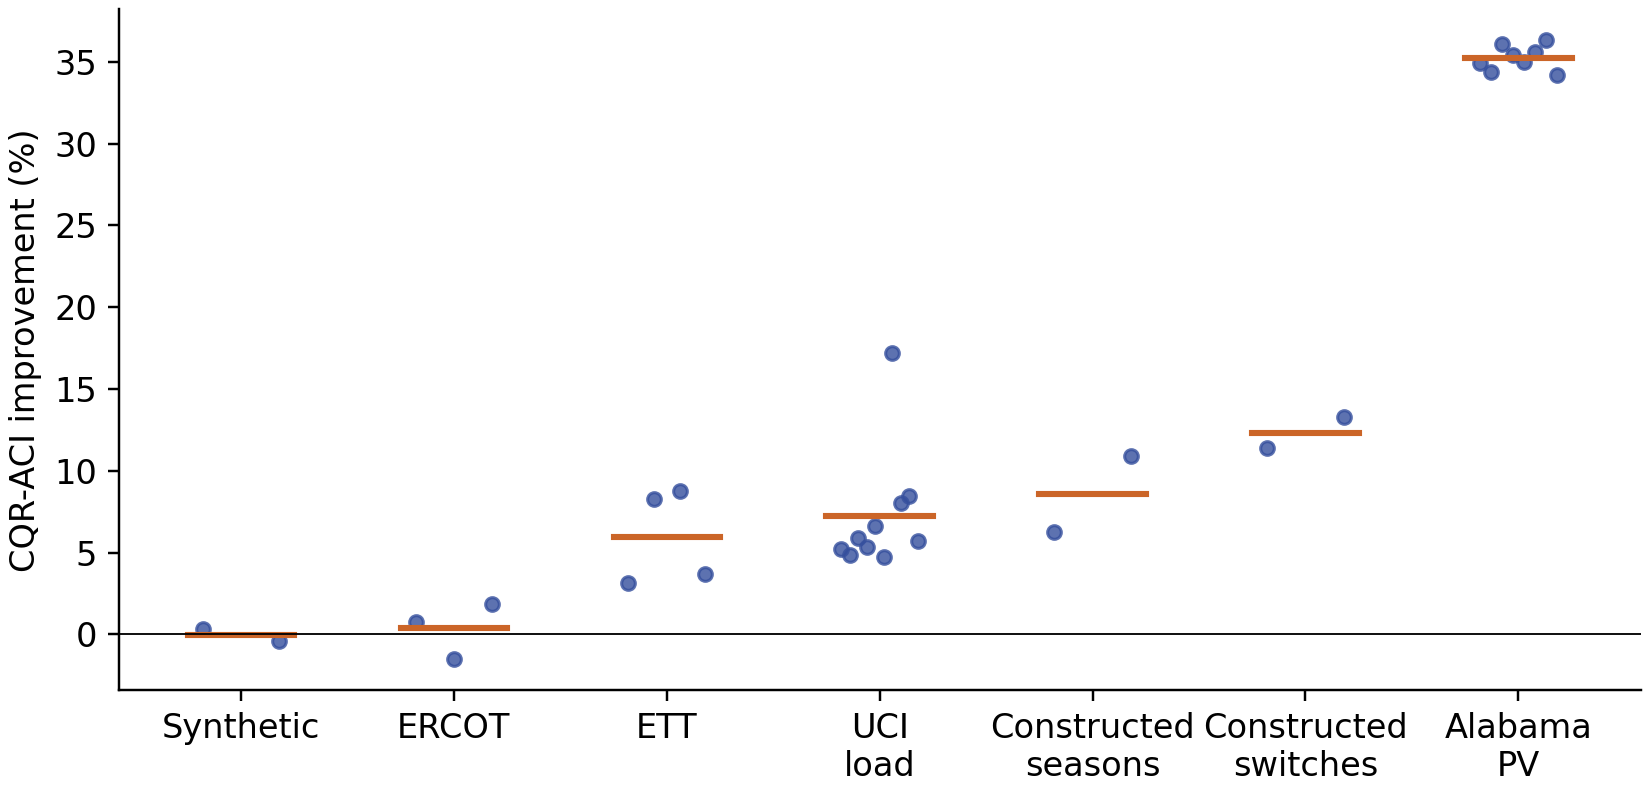
\includegraphics[width=\textwidth]{figures/families.png}
\caption{Each point is one series averaged across four backbones; horizontal orange marks
are family means. Constructed and synthetic series remain visible rather than being
counted as independent observed energy systems.}\label{fig:families}\end{figure}

Per-backbone mean gains are 15.15\% for Chronos-2, 13.82\% for Chronos-Bolt, 12.90\%
for Moirai and 12.41\% for the archived TimesFM configuration. On the separate GEFCom
panel, CQR--ACI gains 19.63\% overall: 41.46\% for solar and 13.08\% for wind, with
89.99\% mean coverage. This is evidence beyond the Alabama solar panel, but does not
convert correlated zones into independent geographic samples.

At block lengths 100, 200 and 400, 109 primary pairs have a positive paired-bootstrap
95\% interval and two have a negative interval. The centered-test/BH procedure identifies
109 positive and two negative differences at each of these block lengths. These counts
are reported with the dependence caveat above; the magnitude and family distribution of
the effect remain the main empirical evidence.

\subsection{Delayed feedback makes rule choice consequential}
Figure~\ref{fig:horizon} and Table~\ref{tab:horizon} show the joint horizon/feedback
experiment. At $h=24$, CQR--ACI has 87.34\% mean coverage, compared with 87.10\% for
residual--ACI. CQR--PI-log attains 89.96\% coverage and a 17.09\% score improvement
relative to residual--ACI, compared with 13.15\% for CQR--ACI. CQR--ACI's average number
of clipped updates, counting validation and test adaptation, increases from 3.06 at
$h=1$ to 201 at $h=24$. This is consistent with the projection term in
Equation~\eqref{eq:identity}, although a count alone does not measure its signed magnitude.

\begin{figure}[htbp]\centering
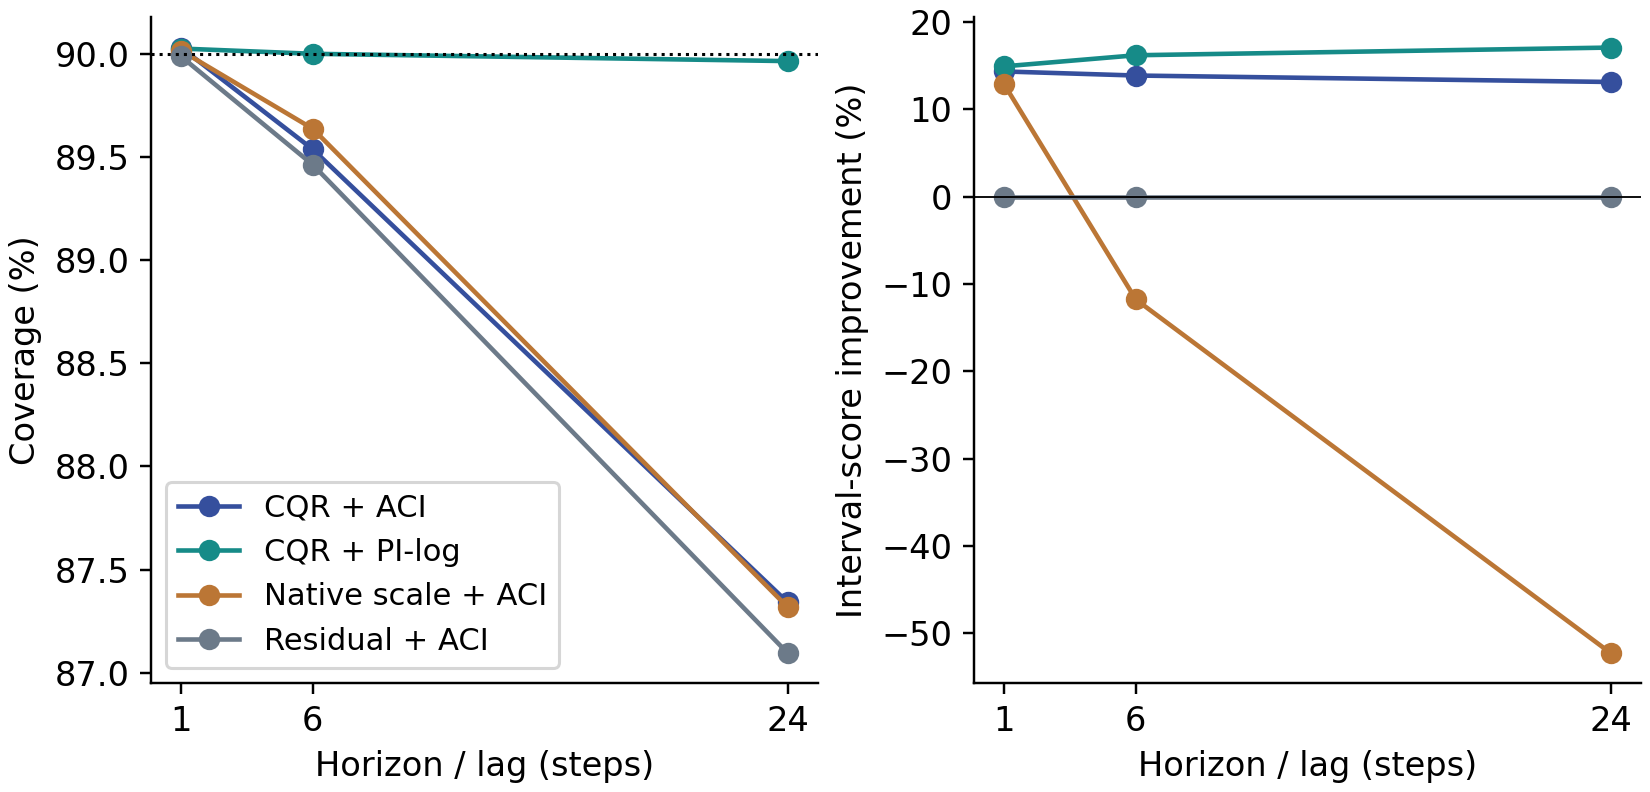
\includegraphics[width=\textwidth]{figures/horizon.png}
\caption{Joint changes in horizon and natural feedback delay on eight series and two
Chronos models. Coverage is an average; score gains use the horizon-specific residual--ACI
denominator. Solar steps are ten minutes, so $h=24$ is not day-ahead for those series.}
\label{fig:horizon}\end{figure}

The PI result is not a claim of uniformly improved reliability. At $h=24$, its local
150-origin coverage error is 4.86 percentage points, versus 4.52 for CQR--ACI. Improved
overall coverage can coexist with worse local variation. The controller also emits some
singletons after negative signed corrections: CQR--PI-log's average singleton rate is
0.567\% at $h=24$, versus 0.048\% for CQR--ACI. No infinite test intervals occur for
these two reported variants in this panel.

The fixed-forecast intervention separates lag from changing forecast difficulty
(Figure~\ref{fig:delay}). On the same $h=1$ predictions, increasing calibration lag from
1 to 24 steps changes residual--ACI coverage from 89.99\% to 88.62\% and CQR--ACI from
90.03\% to 89.52\%. CQR--PI-log remains at 89.99\% for lag 24, while its local coverage
error is 2.88 percentage points compared with 2.08 for CQR--ACI. Thus feedback restriction
alone can alter the relevant coverage comparison. The larger deficit in true $h=24$
forecasts additionally reflects changes in the forecast/score stream; lag alone does not
explain its entire magnitude.

\begin{figure}[htbp]\centering
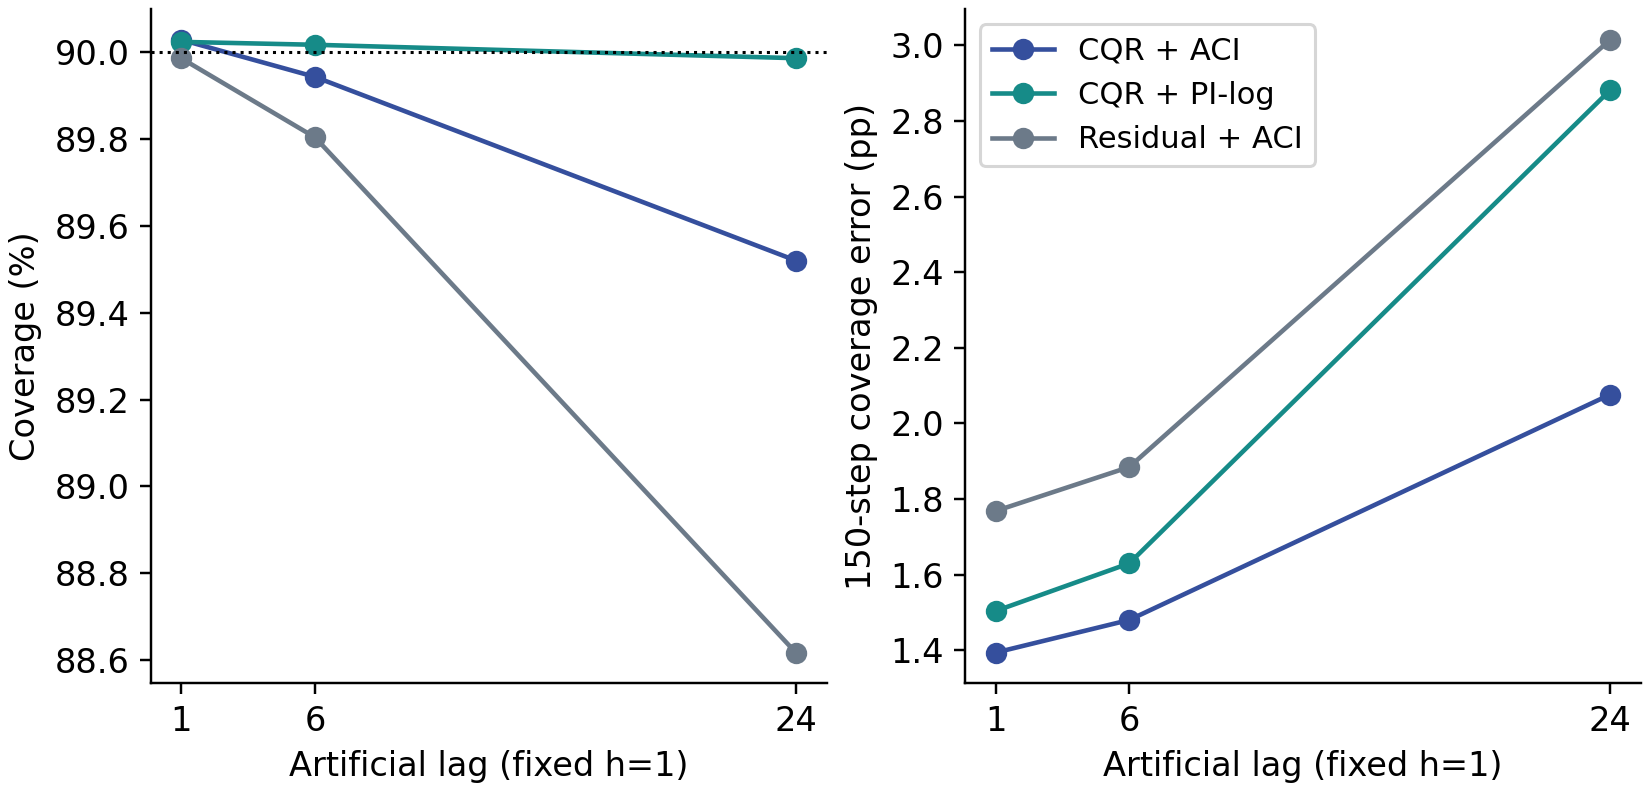
\includegraphics[width=\textwidth]{figures/delay_control.png}
\caption{Exploratory intervention holding one-step predictions and targets fixed while
withholding calibration outcomes. Overall coverage and local coverage error respond
differently. This isolates the calibrator's feedback channel, not the model's context.}
\label{fig:delay}\end{figure}

\subsection{Earlier long-horizon PV diagnostics}
The separate long-horizon diagnostic concerns two other development photovoltaic
series and two backbones, so it is not a within-panel comparison with the one-step
decomposition.
On the two development photovoltaic series and two backbones, tuned CQR--COP at
$h=24$ attains 90.41\% overall coverage, yet only 79.93\% on positive-output targets
and 97.05\% on zero-output targets (Figure~\ref{fig:solarconditional}). Zero outputs
constitute approximately 61.04\% of these test segments. At $h=1$ and $h=6$,
positive-output coverage is 87.95\% and 82.42\%, respectively, despite overall coverage
near 90\%. These are four model--series pairs from two series, not four independent
solar datasets. Positive output is an outcome-defined diagnostic and need not
coincide with astronomical daytime. A marginal coverage theorem does not promise
coverage on this subset, so the finding is not a counterexample to that theorem.

\begin{figure}[!htbp]\centering
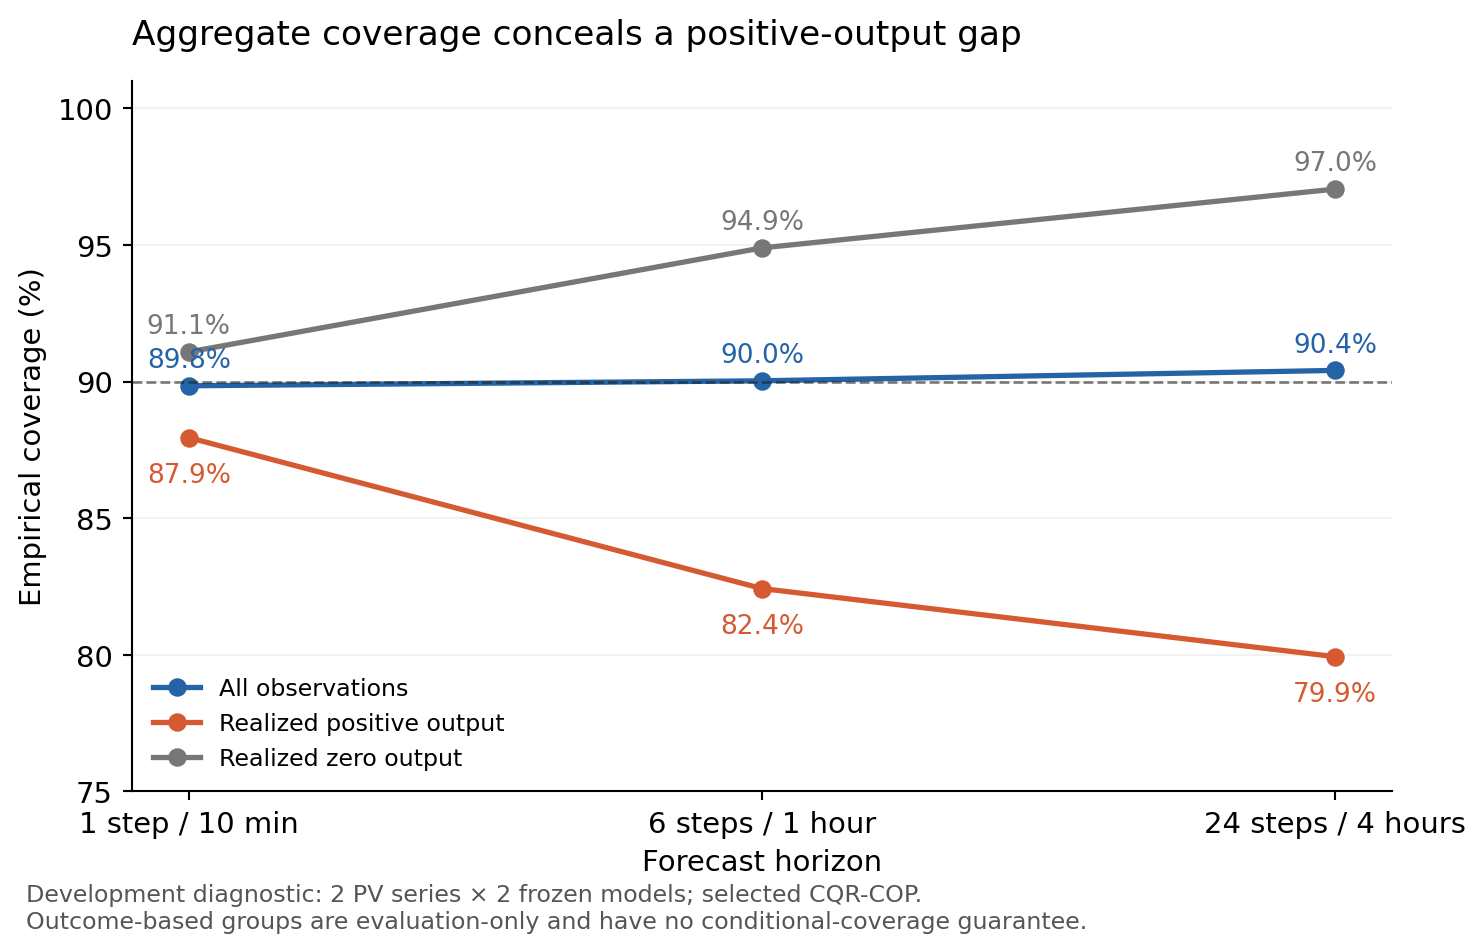
\includegraphics[width=\textwidth]{figures/solar_conditional_coverage.png}
\caption{Post-hoc photovoltaic reliability diagnostic for selected CQR--COP.
Coverages average over two series and two models. The zero/positive labels are used
only for evaluation; prediction and validation never use the future target label.
At this sampling rate, 24 steps represent four hours.}
\label{fig:solarconditional}\end{figure}

The observable-width grouping experiment tests whether a simple existing approach
can reduce the deficit. Separating both memory and state increases positive-output
coverage from 78.93\% to 83.49\% relative to matched shared-state CQR on these solar
pairs. Overall coverage changes from 88.46\% to 89.45\%, with a 2.47\% interval-score
gain. The positive-output gap remains substantial. Separating memory alone improves
solar interval score by 6.75\% but reduces overall coverage to 85.66\%, illustrating
why a proper-score change should be accompanied by coverage diagnostics.
Across all 16 development pairs, the both-grouped CQR gain is only 1.12\%.
On the confirmation families, the same grouping yields a 3.27\% gain at $h=24$,
but coverage remains 88.56\%, compared with 87.87\% for shared ACI. Grouping is thus
an informative control, not a demonstrated solution to conditional reliability.




\section{Detailed score constructions and original comparisons}\label{app:details}
\subsection{Scores and inversions}
Let $b_t=u_t-\ell_t$. We construct an outcome scale $v_t$ from a causal exponentially
weighted mean absolute error, updated only when a target is revealed, with decay 0.05.
Its initialization uses the first available forecast band and point prediction, not an
unseen outcome. The scale is bounded below by $10^{-12}$ for numerical arithmetic.
Define $\tilde b_t=\max(b_t,10^{-3}v_t)$. The four primary scores are
\begin{align}
 s_t^{\rm R}&=|y_t-m_t|,&
 s_t^{\rm E}&=|y_t-m_t|/v_t,\\
 s_t^{\rm N}&=|y_t-m_t|/\tilde b_t,&
 s_t^{\rm Q}&=\max(\ell_t-y_t,y_t-u_t).
\end{align}
They yield intervals $[m_t-q_t,m_t+q_t]$, $[m_t-v_tq_t,m_t+v_tq_t]$,
$[m_t-\tilde b_tq_t,m_t+\tilde b_tq_t]$ and $[\ell_t-q_t,u_t+q_t]$, respectively.
The native-scale control asks whether a native width helps without using native endpoints
directly; the past-error-scale control asks whether a simple outcome-based scale suffices.
CQR thresholds may be negative, allowing a band to shrink.

If inversion produces reversed endpoints, we record the event and emit a singleton at
their center. This is a practical interval repair rather than the exact empty set obtained
from signed-score inversion. Coverage-driven updates use the emitted interval. Infinite
intervals, if produced, are counted and retain infinite interval scores; they are not
capped or dropped. The primary CQR--ACI test intervals are singletons at an average rate
of 0.013\%, and no infinite intervals occur in the reported primary comparison.

We also examine normalized CQR, with denominator
$\max(b_t+\lambda v_t,10^{-3}v_t)$ for $\lambda\in\{0,0.01,0.1,0.5,1\}$.
A prefix selector chooses the lowest validation interval score among these five recipes
and the four primary scores under ACI. This is an existing model-selection principle used
as a diagnostic, not a proposed novel algorithm. A separate midpoint control replaces
$m_t$ by $(\ell_t+u_t)/2$ while retaining the residual or native-scale score.


\begin{table}[!htbp]\centering\small
\caption{Original one-step main-panel methods. Gain uses default residual--ACI;
Gap and Local denote absolute overall and 150-origin coverage errors in percentage points.}
\label{tab:main}\begin{tabular}{lrrrr}
\toprule
Score / rule & Gain (\%) & Cov. (\%) & Gap (pp) & Local (pp) \\
\midrule
residual/aci & 0.00 & 89.94 & 0.07 & 1.66 \\
error-scale/aci & 2.17 & 90.00 & 0.03 & 1.06 \\
native-scale/aci & 11.50 & 89.98 & 0.05 & 1.42 \\
cqr/aci & 13.57 & 89.98 & 0.05 & 1.45 \\
residual/faci & 8.57 & 89.19 & 0.81 & 1.86 \\
cqr/faci & 14.87 & 89.49 & 0.52 & 1.71 \\
residual/saocp & 3.32 & 92.54 & 2.64 & 2.92 \\
cqr/saocp & 12.40 & 90.73 & 1.49 & 2.07 \\
cqr/pi-log & 13.88 & 90.00 & 0.06 & 1.51 \\
cqr/sfogd & 13.28 & 90.00 & 0.03 & 0.98 \\
prefix-selected/aci & 13.72 & 89.98 & 0.05 & 1.46 \\
residual/aci/tuned & 5.23 & 89.74 & 0.28 & 1.65 \\
cqr/aci/tuned & 14.18 & 89.92 & 0.15 & 1.74 \\
\bottomrule
\end{tabular}\end{table}
\begin{table}[!htbp]\centering\scriptsize
\caption{Earlier CQR rate sensitivity at $h=24$. Development and traffic/exchange-rate
panels each have 16 pairs. S/I denote shared/issued. Selection uses validation only.}
\label{tab:rates}\begin{tabular}{llrrrrrr}
\toprule
Panel & Grid & Gain & Wins & Cov. S & Cov. I & Local S & Local I \\
\midrule
Development & original & 6.54 & 15/16 & 88.18 & 89.56 & 5.33 & 5.55 \\
Development & scaled & 0.73 & 13/16 & 89.54 & 89.35 & 5.62 & 5.60 \\
Development & wide & 0.59 & 13/16 & 89.45 & 89.32 & 5.66 & 5.61 \\
Traffic/FX & original & 8.43 & 16/16 & 87.87 & 89.43 & 5.79 & 6.12 \\
Traffic/FX & scaled & 1.27 & 13/16 & 89.00 & 89.03 & 6.14 & 6.25 \\
Traffic/FX & wide & 0.99 & 13/16 & 88.78 & 89.01 & 6.21 & 6.22 \\
\bottomrule
\end{tabular}
\end{table}
\begin{table}[!htbp]\centering\scriptsize
\caption{Original one-step PV decomposition. Contributions use each pair's overall
residual denominator and add to its overall gain; group gains use group denominators.}
\label{tab:solarparts}\begin{tabular}{llrrrrr}
\toprule
Settings & Group & Share & Gain & Contribution & Cov. R & Cov. CQR \\
\midrule
default & all & 100.00 & 35.25 & 35.25 & 89.88 & 89.96 \\
default & positive & 38.84 & 21.32 & 15.61 & 74.38 & 84.96 \\
default & zero & 61.16 & 73.37 & 19.64 & 99.72 & 93.14 \\
tuned & all & 100.00 & 20.51 & 20.51 & 89.34 & 89.72 \\
tuned & positive & 38.84 & 12.77 & 10.43 & 80.17 & 86.32 \\
tuned & zero & 61.16 & 54.89 & 10.08 & 95.16 & 91.88 \\
\bottomrule
\end{tabular}
\end{table}
\section{Detailed new-source protocol and reference comparison}\label{app:newprotocol}
\subsection{Protocol-locked confirmation on two new sources}\label{sec:newdesign}
After the preceding sensitivities, we fixed an additional protocol before numeric data
acquisition or calibration inspection. It selects MPI-BGC Jena roof temperature and
pressure for the first 3,600 hours of 2026, and PM2.5 at the Aotizhongxin and Dingling
stations for the first 3,600 hours from 1 March 2013 in the UCI Beijing archive
\citep{jena2026weather,chen2017air}. These are four series from two sources, evaluated
with the same two cached Chronos checkpoints: eight dependent model--series pairs.
Both models emit all 24 horizons at 2,976 consecutive origins. The main test segment
has 1,776 origins before excluding missing targets. Context length, batch size, dtype,
checkpoint-file hashes, timestamps and generation code are recorded for every archive.

Missing input observations are forward filled causally; missing targets are excluded
from score memory, controller increments and evaluation. Windows contain the latest
$W$ observed, revealed scores. Issued-state phases continue without an increment when
their outcome is missing. Local coverage uses 150 calendar-origin windows with their
observed denominators. The weather forecast targets are complete; the one missing
initial weather hour precedes all forecast contexts. The new-source protocol is locally
timestamped and hashed, not externally preregistered. Public historical air-quality data
may have been used in neural pretraining; new-to-calibration does not imply unseen-to-model.

For both scores and states, nested grids comprise the original rates at $W=450$;
the wide grid described below; and that grid augmented with zero
and four smaller rates ($10^{-6}$, $5\times10^{-6}$, $10^{-5}$ and $5\times10^{-5}$).
The final stage crosses these expanded rates with $W\in\{200,450,900\}$. Validation selects the minimum interval
score, breaking ties toward smaller rate and then window. Zero-rate trajectories
provide both fixed-window and selected-window rolling controls. Early and late
validation intervals, $[600+h-1,900-h+1)$ and $[900,1200-h+1)$, probe selector
stability without changing the primary full-validation selector or test segment.

The wide grid combines rates 0.0001, 0.0002, 0.0005, 0.001, 0.002, 0.005,
0.01, 0.02, 0.05 and 0.1 with the three original rates divided by $h$.

The predefined complete-weather subset also receives full AcMCP scorecasting: the
pinned author's MA$(h-1)$ plus cross-horizon regression implementation, at all horizons
1--24, with its supported CSS fitting option. We identify it as AcMCP-CSS, not the
default CSS-ML configuration. Rolling history is 600, $C_{\rm sat}=0.5$, and $K_I$
uses only the first 600 revealed target-clock error rows. The rate grid is
$\{0.001,0.005,0.01,0.05,0.1\}$ and these rates divided by $h$; the same validation
block selects it. Fitted scorecasts are independent of this rate, so they are cached
once per archive. A cached interval replay must agree with every original R trajectory
at rate 0.01 before evaluating the other rates. A matched no-scorecast PID control
uses the identical rate grid. Both are signed-error complete configurations; their
comparison to native CQR does not isolate controller quality.

\subsection{PV support and asymmetric-residual controls}\label{sec:pvcontrol}
On all 32 original one-step PV pairs, we additionally compare the established
signed-error construction
$[m_t+Q_{a_t/2}(Y-m),m_t+Q_{1-a_t/2}(Y-m)]$ with symmetric residuals and CQR.
It shares the total-miscoverage ACI state, timing and window. Each construction
uses the original nine rate/window settings; fixed defaults and a separately selected
zero-rate rolling control are retained. This is exploratory analysis of previously
inspected data, distinct from the new-source confirmation.

All three constructions are evaluated raw and after the same known-support projection
$[L,U]\mapsto[\max(0,L),\max(0,U)]$. Projected and raw configurations are separately
selected on validation score, while each candidate keeps its raw feedback trajectory:
the projection isolates interval geometry and is not a new feedback algorithm.
For a nonnegative target and finite ordered endpoints, projection cannot worsen
interval score or lose a covered target. In particular, when $L<0\leq U$, score
improvement is exactly $-L$, with unchanged coverage. When $U<0$, both endpoints
become zero and previously uncovered zeros can become covered. We therefore report
coverage changes as well as width and miss-distance penalties.

In addition to actual zero/positive targets, an observable grouping compares each point
forecast with the median of the first 600 point forecasts. This threshold is fixed
before validation; the high-forecast group is known at issue time and is not selected
using the future outcome. It is a diagnostic control, not a conditional-validity guarantee.

\begin{table}[!htbp]\centering\small
\caption{Original configured weather comparison using full validation. Ratios use
window-selected Rolling CQR; this precedes the common-history sensitivity.}
\label{tab:acmcpfull}\begin{tabular}{rlrrr}
\toprule
Horizon & Method & IS ratio & Coverage & Local \\
\midrule
1 & Rolling CQR & 1.000 & 89.37 & 3.15 \\
1 & Issued CQR & 0.996 & 89.44 & 1.43 \\
1 & AcMCP-CSS & 1.024 & 89.23 & 2.03 \\
1 & PID, no scorecast & 1.026 & 89.20 & 1.99 \\
6 & Rolling CQR & 1.000 & 90.27 & 2.91 \\
6 & Issued CQR & 1.002 & 90.44 & 2.91 \\
6 & AcMCP-CSS & 1.087 & 88.65 & 3.03 \\
6 & PID, no scorecast & 1.084 & 88.39 & 3.23 \\
24 & Rolling CQR & 1.000 & 89.51 & 6.03 \\
24 & Issued CQR & 1.000 & 89.43 & 6.01 \\
24 & AcMCP-CSS & 1.147 & 87.54 & 7.49 \\
24 & PID, no scorecast & 1.056 & 87.18 & 7.31 \\
\bottomrule
\end{tabular}
\end{table}
\section{Post-review temporal and history controls}\label{app:focused}
These analyses revisit inspected data. For positive-rate selectors, each state
minimizes the original full-validation score over the original stored positive
rates, then selects its window when allowed. The smallest rate is $10^{-6}$.
No candidate is added after test inspection. The air-quality CQR gaps are 0.0017\%
at $W=450$ and 0.0021\% with selected memory before admitting zero; these differences
are practically negligible. The paired records retain all rates and score scales.

Each test block contains 592 forecast origins. Missing labels are excluded using
the fixed observed mask. Local errors use 150-origin windows wholly within each
block, so whole-test local error is not exactly the weighted average of block values.
No configuration is reselected on a test block. Figure~\ref{fig:temporal} includes
every source, model and block; early/late validation sensitivity is a different analysis.
\begin{figure}[!htbp]\centering
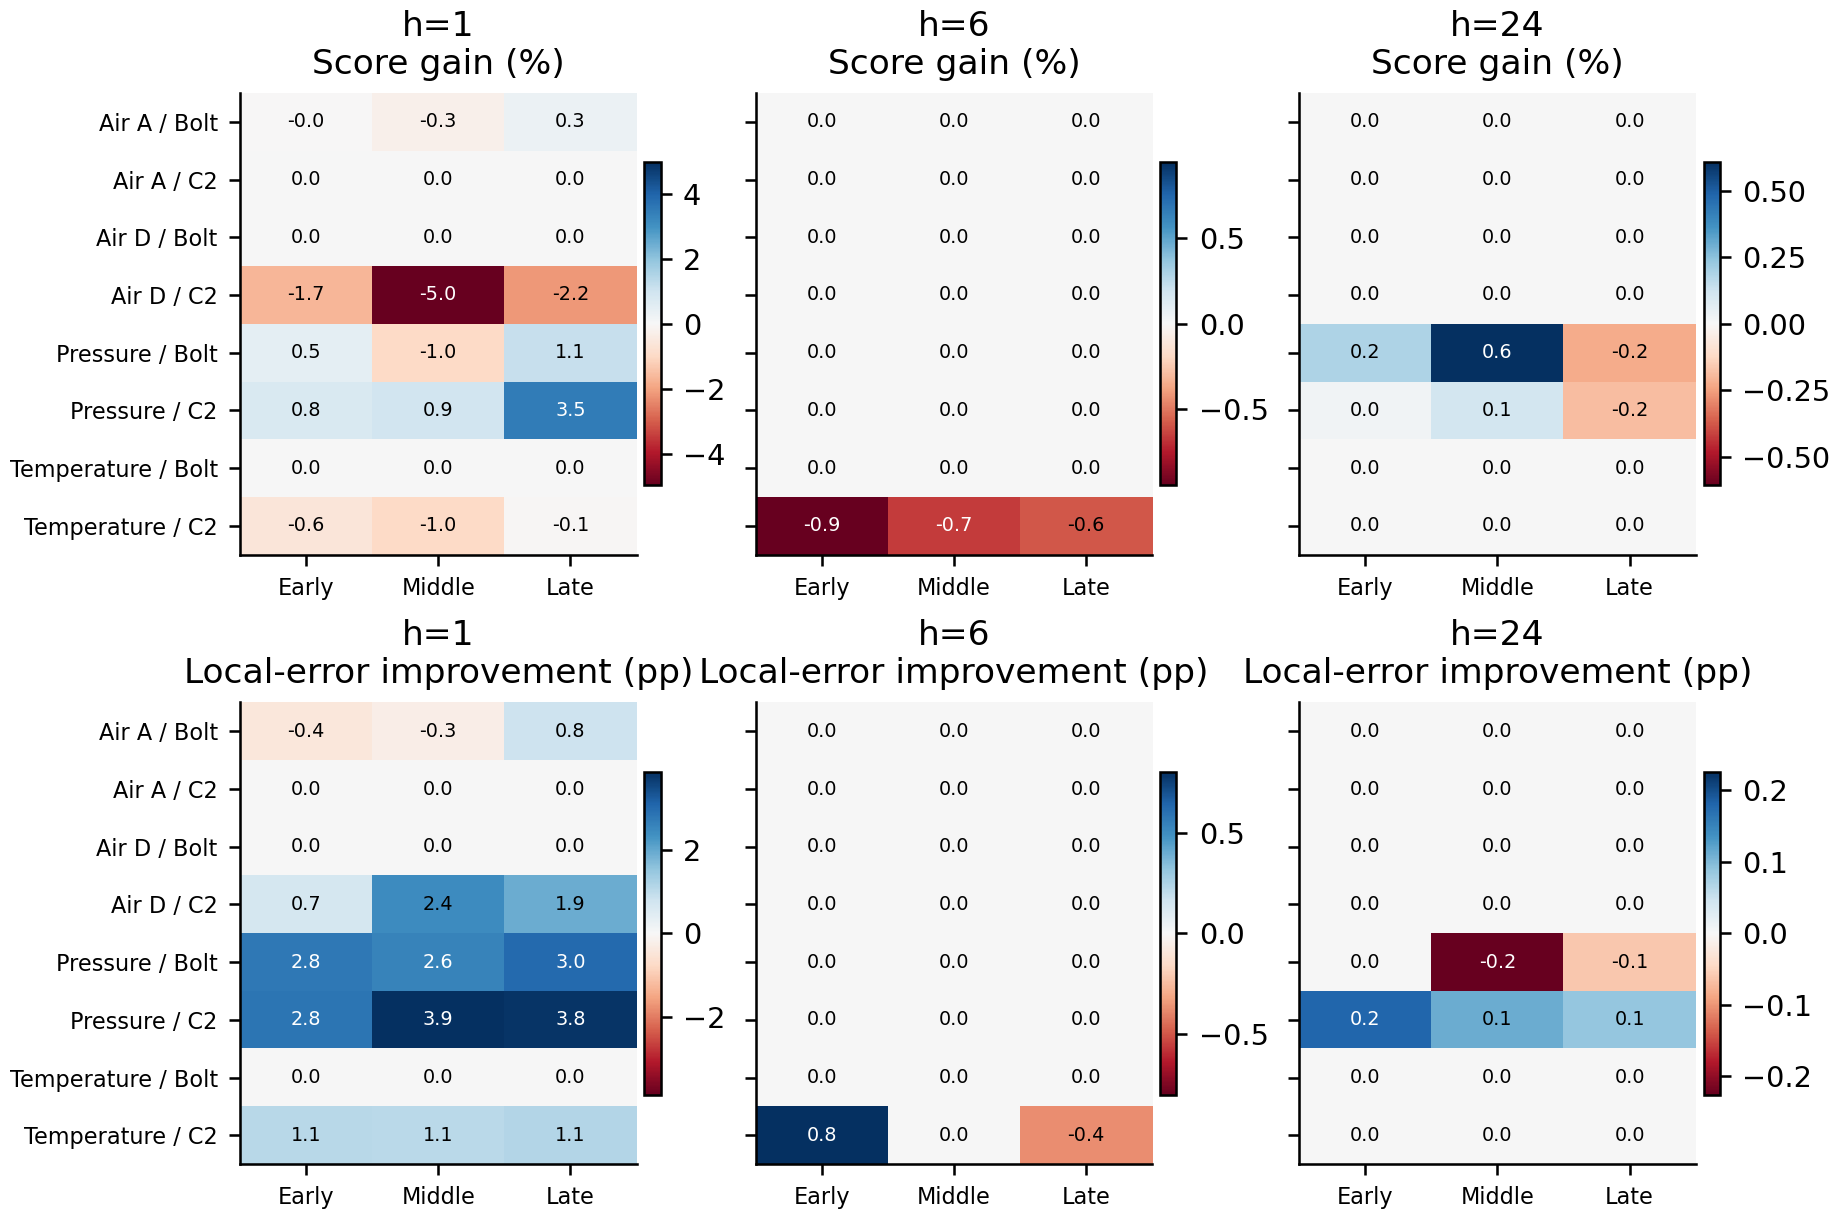
\includegraphics[width=\textwidth]{figures/temporal_pairs.png}
\caption{All eight new-source pairs, three consecutive test blocks. Positive means
issued CQR improves on matched selected-window Rolling CQR. Color scales differ
between panels; values are descriptive, without independent-replication error bars.}
\label{fig:temporal}\end{figure}

The common-history sensitivity adds unmodified author AcMCP-CSS at
$n_{\rm cal}=450$ to the saved $600$ runs. Both use $K_I$ from the first 600
revealed target-clock errors. Because history also changes startup, every method
uses post-startup validation $[900+h-1,1200-h+1)$ and unchanged testing
$[1200,2976)$. All evaluated scorecasts are finite. Each history selects its rate;
joint selection considers both histories. CQR retains its zero/small-rate grid;
PID uses AcMCP's rates with zero scorecasts. Each ratio uses its matched Rolling
denominator. History 900 and CSS-ML are outside this sensitivity.

All 60 sampled history-450 scorecast refits reproduce stored values. Three emit
an MA non-invertibility warning under CSS but return finite predictions. Their
warnings and trajectories are retained. These results characterize the stated
configuration, not default CSS-ML or every AcMCP setting.
\begin{table}[!htbp]\centering\scriptsize
\caption{Complete history sensitivity on all four weather pairs. IS ratios are
averaged after pairing. Coverage is percent and Local is percentage points.}
\begin{tabular}{rllrrr}
\toprule
Horizon & History & Method & IS ratio & Coverage & Local \\
\midrule
1 & 450 & Rolling-CQR & 1.000 & 89.64 & 3.32 \\
1 & 450 & CQR-shared & 0.993 & 89.68 & 1.63 \\
1 & 450 & CQR-issued & 0.993 & 89.68 & 1.63 \\
1 & 450 & AcMCP-CSS & 1.023 & 89.25 & 2.08 \\
1 & 450 & PID-no-scorecast & 1.024 & 89.32 & 1.86 \\
1 & 600 & Rolling-CQR & 1.000 & 89.64 & 3.44 \\
1 & 600 & CQR-shared & 0.995 & 89.60 & 1.71 \\
1 & 600 & CQR-issued & 0.995 & 89.60 & 1.71 \\
1 & 600 & AcMCP-CSS & 1.023 & 89.15 & 2.09 \\
1 & 600 & PID-no-scorecast & 1.024 & 89.32 & 1.86 \\
1 & 450/600 & Rolling-CQR & 1.000 & 89.58 & 3.40 \\
1 & 450/600 & CQR-shared & 0.994 & 89.58 & 1.72 \\
1 & 450/600 & CQR-issued & 0.994 & 89.58 & 1.72 \\
1 & 450/600 & AcMCP-CSS & 1.023 & 89.33 & 1.98 \\
1 & 450/600 & PID-no-scorecast & 1.024 & 89.32 & 1.87 \\
6 & 450 & Rolling-CQR & 1.000 & 89.74 & 2.91 \\
6 & 450 & CQR-shared & 1.018 & 89.96 & 2.45 \\
6 & 450 & CQR-issued & 1.004 & 89.85 & 2.97 \\
6 & 450 & AcMCP-CSS & 1.087 & 88.68 & 3.04 \\
6 & 450 & PID-no-scorecast & 1.087 & 88.84 & 2.97 \\
6 & 600 & Rolling-CQR & 1.000 & 89.95 & 2.83 \\
6 & 600 & CQR-shared & 1.014 & 90.15 & 2.58 \\
6 & 600 & CQR-issued & 1.008 & 90.06 & 2.68 \\
6 & 600 & AcMCP-CSS & 1.085 & 88.67 & 3.09 \\
6 & 600 & PID-no-scorecast & 1.091 & 88.94 & 2.97 \\
6 & 450/600 & Rolling-CQR & 1.000 & 89.96 & 2.86 \\
6 & 450/600 & CQR-shared & 1.029 & 90.09 & 2.24 \\
6 & 450/600 & CQR-issued & 1.004 & 90.20 & 2.79 \\
6 & 450/600 & AcMCP-CSS & 1.085 & 88.67 & 3.09 \\
6 & 450/600 & PID-no-scorecast & 1.091 & 88.94 & 2.97 \\
24 & 450 & Rolling-CQR & 1.000 & 89.32 & 6.33 \\
24 & 450 & CQR-shared & 1.136 & 83.22 & 8.96 \\
24 & 450 & CQR-issued & 1.000 & 89.27 & 6.34 \\
24 & 450 & AcMCP-CSS & 1.138 & 89.18 & 6.45 \\
24 & 450 & PID-no-scorecast & 1.061 & 88.20 & 6.49 \\
24 & 600 & Rolling-CQR & 1.000 & 89.44 & 6.75 \\
24 & 600 & CQR-shared & 1.039 & 87.43 & 7.42 \\
24 & 600 & CQR-issued & 1.000 & 89.43 & 6.74 \\
24 & 600 & AcMCP-CSS & 1.172 & 89.27 & 6.27 \\
24 & 600 & PID-no-scorecast & 1.067 & 88.37 & 6.43 \\
24 & 450/600 & Rolling-CQR & 1.000 & 89.44 & 6.75 \\
24 & 450/600 & CQR-shared & 1.039 & 87.43 & 7.42 \\
24 & 450/600 & CQR-issued & 1.000 & 89.43 & 6.74 \\
24 & 450/600 & AcMCP-CSS & 1.164 & 89.18 & 6.48 \\
24 & 450/600 & PID-no-scorecast & 1.065 & 88.60 & 6.24 \\
\bottomrule
\end{tabular}
\end{table}


\clearpage
\bibliographystyle{elsarticle-num-names}
\bibliography{references}
\end{document}
